\documentclass{article}
\usepackage[utf8]{inputenc}
\usepackage{amsmath}
\usepackage{amsfonts}
\usepackage{amsthm}
\usepackage{amssymb}
\usepackage{enumitem}
\usepackage{graphicx}
\graphicspath{ {./imgs/} }
\usepackage[margin=1in]{geometry}
\usepackage{float}
\usepackage{xcolor}
\usepackage{color}
\usepackage[landscape]{geometry}
\usepackage{hyperref}
\usepackage{listings}
\hypersetup{
    colorlinks=true, 
    linktoc=all,     
    linkcolor=blue,  
}
\newcommand\todo[1]{\textcolor{red}{TODO: {#1}}}

\title{MAT137 - Summer 2022 Notes}
\author{}
\date{}

\begin{document}

\maketitle

\tableofcontents

\newpage
\section{Sets, Quantifiers, and Conditionals}
\subsection{Symbols, Quantifiers, and Conditionals}
\\
\textbf{Logical symbols}\\
$\land$ = ``and" \ |  \ Exclusive\\
$\lor$ = ``or" \ | \ Inclusive\\
$\neg$ = ``not'' \ | \ Negation
\begin{center}
\begin{tabular}{ c|c|c|c } 
 A & B & $ A \land B$ & A $\lor$ B\\
 \hline
 T & T & T & T \\ 
 T & F & F & T\\
 F & T & F & T \\
 F & F & T & F\\
 % 
\end{tabular}
\end{center}
\\ \textbf{Quantifiers}\\
$\forall$ = Universal quantifier (For all)\\
$\exists$ = Existential quantifier (There exists)\\
The negation of $\forall$ is $\exists$; the negation of $\exists$ is $\forall$.\\
\\
\textbf{Conditionals}\\
$\implies$ = Implies \ | \ (If A, then B)\\
$\iff$ = Biconditional (If and only if) \ | \ (A $\implies$ B) $\land$ (B $\implies$ A)
\begin{center}
\begin{tabular}{ c|c|c|c } 
 A & B & $ A \implies B$ & A $\iff$ B\\
 \hline
 T & T & T & T \\ 
 T & F & F & F\\
 F & T & T & F \\
 F & F & F & T\\
 % 
\end{tabular}
\end{center}
\subsection{Logically Equivalent Statements}\\
If two statements are \textbf{logically equivalent}, they will have the same true/false values. For example, the negation of A $\implies$ B is logically equivalent to A $\land$ ($\neg$ B).
\\
For the implication A $\implies B$:

    $\neg$B $\implies$ $\neg$A \ | \ Contrapositive
    
    B $\implies$ A \ | \ Converse
    
    $\neg$A $\implies$ $\neg$B \ | \ Inverse

\begin{center}
    \begin{tabular}{ c|c|c|c|c|c }
    A & B & A $\implies$ B & $\neg$B $\implies$ $\neg$A & B $\implies$ A & $\neg$A $\implies$ $\neg$B\\
    \hline
    T & T & T & T & T & T\\
    T & F & F & F & T & T\\
    F & T & T & T & F & F\\
    F & F & T & T & T & T
    \end{tabular}
\end{center}
\\ \subsection{Examples of Logical Statements}
\begin{enumerate}
    \item \textbf{Students on fire}\\
    ``No two students in this class are not on fire'', written using logical symbols is:\\
$\forall$x, y $\in S$, $(F(x) \land F(y))$\\\\
To find the negation, we can write:\\
$\exists$x, y $\in S$, $\neg(F(x) \land F(y))$\\
In English, we would say, ``There exists a pair of students in the class that not are on fire.''
\end{enumerate}


\subsection{Sets}
\textbf{Sets} are collections of elements: we use set builder notation to mathematically describe them.\\
For example, the \textbf{set of even numbers} is written as:
$\{ \forall n \in \mathbb{Z} : \exists a \in \mathbb{Z}, n = 2a \}$\\
In other words, it is the set of all integers $n$ such that for some value $a$, $n$ is a multiple of $2a$.\\
\\
\textbf{Notation}\\
$\cup$ = Union \ | \ The set of items that are in the set A or B: $A \cup B = \{x : x \in A \lor x \in B \}$\\
$\cap$ = Intersection \ | \ The set of items that are in the set A and B: $A \cap B = \{x : x \in A \land x \in B \}$\\
$\emptyset$ = Empty Set \ | \ A set that contains no elements. If the set is empty, then it is implied that $\forall x \in \emptyset, x$ is true.
\\
\\
\textbf{Symmetric Differences}\\
Given two sets A and B, we can define:\\
$A \setminus B = \{ x \in A : x \not \in B \}$ \ | \ Set minus: The items in A that are not in B.\\
$A \triangle B = (A \setminus B) \cup (B \setminus A)$ \ | \ Symmetric Difference: The items that are not in both A and B (the union of two sets excluding the intersection).\\
Symmetric differences are also called disjunctive unions, and can be expressed using the XOR operation $\oplus$.
\begin{figure}[h]
    \centering
    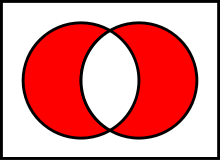
\includegraphics[scale=0.4]{imgs/xor1.png}
    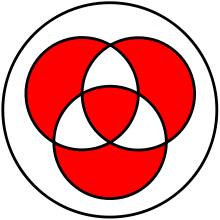
\includegraphics[scale=0.31]{imgs/xor2.png}
    \caption{Visual representation of $A \triangle B$, and $(A \triangle B)\triangle C$.}
\end{figure}
\\
\\
\textbf{Double Quantifiers}\\
For multiple quantifiers, the order is very important. For example, let $S(x,y)$ = ``$x$ studies with $y$'', where $x,y \in$ \{Students\}. Depending on how we quantify $x$ and $y$, we get:
\begin{enumerate}
    \item $\forall x, \forall y, S(x,y)$ \ | \ Every student studies with everyone.
    \item $\forall x, \exists y, S(x, y)$ \ | \ Every student studies with at least one student.
    \item $\exists x, \forall y, S(x, y)$ \ | \ There exists a student that studies with everyone.
    \item $\exists x, \exists y, S(x, y)$ \ | \ There exists a student that studies with at least one student.
\end{enumerate}

\section{Functions}
\subsection{Injective Functions}
Injective functions are ``one-to-one'', meaning that different x values produce different f(x) values.\\
In other words, a function $f: A \rightarrow B$ is injective $\iff$ $\forall x_1, x_2 \in A, x_1 \neq x_2 \implies f(x_1) \neq f(x_2)$\\
Equivalently, $\forall x_1, x_2 \in A, f(x_1) = f(x_2) \implies x_1 = x_2$.
\subsubsection{Proving Injectivity}
Determine whether $f(x) = 2x^3 + 7$ is injective or not.
\begin{proof}
We want to show that $\forall x, y \in \mathbb{R}, f(x_1) = f(y) \implies x = y$. Let $x, y \in \mathbb{R}$. Assume $f(x) = f(y)$. So, we must show that $x = y$.\\\
\begin{align*}
    & 2x^3 + 7 = 2y^3 + 7 & \text{ by assumption}\\
    \implies & 2x^3 = 2y^3 & \text{using arithmetic}\\
    \implies & \frac{2x^3}{2} = \frac{2y^3}{2}\\
    \implies & (x^3)^\frac{1}{3} = (y^3)^\frac{1}{3}\\
    \implies & x = y
\end{align*}
So, $f(x)$ is injective.\\
\end{proof}

\subsubsection{Proving Non-Injectivity}
To prove a function $f: A \rightarrow B$ to not be injective, show that $\exists x, y \in A, f(x) = f(y) \land x \neq y$\\
\\
For example, prove that $f(x) = x^2$ is not injective.\\
\begin{proof} Let $f(x) = x^2$. We want to show that $\exists x, y \in \mathbb{R}, x^2 = y^2 \land x \neq y)$.\\
Let $x = 4$ and $y = -4$.\\
We can see that $(4)^2 = (-4)^2$, so $f(x) = f(y)$, but $x \neq y$. \\
Therefore, there exists two x values from the same y value, hence $y = x^2$ is not injective.\\
\end{proof}
\subsubsection{Increasing Functions}
A function $f: A \rightarrow B$ is said to be increasing if for $\forall a < b \in A, f(a) < f(b)$.\\
Similarly, a function is decreasing if for $\forall a < b \in A, f(a) > f(b)$.
\subsection{Theorem: Increasing Functions Implies Injectivity}
Claim. If $f$ is increasing on $A$, then $f$ is injective on $A$.
\begin{proof} Let $a, b \in A$. Assume $f$ is increasing. We want to show  $f$ is injective. Assume $a \neq b$ and show that $f(a) \neq f(b)$.\\
It was assumed that $a \neq b$ implies $a < b \implies f(a) < f(b)$ or $b < a \implies f(b) < f(a)$, since $f$ is increasing. Therefore, $f(a) \neq f(b)$. Thus, if $f$ is increasing, then it is injective.\\
\end{proof}
\subsection{Disproving a Theorem}
Claim. We want to disprove that if $f$ is injective on $A$, then $f$ is increasing.
\begin{proof}
Let $f: A \rightarrow B$ be a function. We want to show that it is not the case that $\forall$ such $f$, injectivity implies increasing.\\
This means that there exists a function that it is injective and not increasing.\\
Let $f(x) = 2 - x$, with $x \in A$.\\
Injectivity: Let $a, b \in A$. If $2 - a = 2 - b$, it is implied that $a = b$.\\
Not increasing: We want to show that $\exists a, b \in A, a < b \land f(a) \geq f(b)$.\\
Let $a = 1, b = 3$, so $1 < b$ and $2 - 1 \geq 2 - 3$.
\begin{align*}
    RHS: & 2 - 3 & LHS: & 2 - 1\\
    & -1 & & 1\\
\end{align*}
$1 \geq -1$, so $f(a) \geq f(b)$. Therefore, $\exists f: A \rightarrow B$ such that $f$ is injective, and $f$ is not increasing.
\end{proof}
\subsection{Floor Functions}
Given an $x \in \mathbb{R}$, we define the \textbf{floor} of $x$, denoted $\lfloor x \rfloor$, as the largest integer $\leq x$. For example:
\begin{align*}
    & \lfloor \pi \rfloor = 3 & &  \lfloor 7.9 \rfloor = 7 & & \lfloor -0.5 \rfloor = -1
\end{align*}
\section{Induction}
\textbf{Induction proofs} are a type of mathematical proof, used to prove a statement $P(n)$ over a countable set (e.g., natural numbers $\mathbb{N})$.
\subsection{Format of Induction Proofs}
\begin{enumerate}
    \item \textbf{Base Case: }Proving the statement for the first possible value for $n$.
    \item \textbf{Hypothesis: }Assuming that statement $P(n)$ is possible for any given $n = k$.
    \item \textbf{Induction Step: }Based on the hypothesis, prove the statement also holds for $n = k = 1$.
\end{enumerate}
\subsection{Example of Induction Proof}
\subsubsection{Example 1: Divisibility}
Show that $n^3 + 2n$ is divisible by $3$ for all positive integers $n$.
\begin{proof}
We WTS $\forall n \in \mathbb{N}, n^3 + 2n = 3x$ for some $x \in \mathbb{Z}$.\\
\\
\textbf{Base Case: }Let $n = 1$. Then, $(1)^3 + 2(1) = 1 + 2 = 3$. Since $3 = 3x$ for $x = 1$, so our base case holds.\\
\\
\textbf{Induction Step: }Assume that $n^3 + 2n = 3x$ be true for $n = k$. We want to show this holds for $n = k + 1$. So:
\begin{align*}
    (k + 1)^3 + 2(k + 1) & \implies (k^3 + 3x^2 + 3k + 1) + 2k + 2 & \text{By expanding.}\\
    & \implies k^3 + 3x^2 + 5k + 3 & \text{Using arithmetic.}\\
    & \implies (k^3 + 2k) + (3k^2 + 3k + 3)\\
    & \implies 3x + 3k^2 + 3k + 3 & \text{Since }k^3 + 2k = 3x\\
    & \implies 3(x + 3k^2 + k + 1) & \text{By factoring 3.}
\end{align*}
Hence, $(k+1)^3 + 2(k+1)$ must be divisible by 3. \\
\\
Therefore, $n^3 + 2n$ is divisible by $3$ for all positive integers $n$.\\
\end{proof}
\section{Absolute Values}
\textbf{Absolute values}, denoted $|n|$, is a value that is always considered 0 or positive.\\
It can be defined as a function $|x|: \mathbb{R} \to \mathbb{R}$ such that: 
$$|x| = \begin{cases}
x & x\geq 0\\
-x & x < 0
\end{cases}$$
\subsection{Determining Absolute Values}
See \hyperlink{http://home.tykenho.com/LectureNotes137_Preview.pdf}{Tyler Holden's 137 Notes} for examples (2.1.1).\\
Generally, break the absolute values into cases of when $x$ will be positive, or when $x$ is negative and we need to multiply the value by $-1$. By determining these cases, we can then either evaluate the absolute value, or determine its inequality to a polynomial.
\subsection{Properties of Absolute Values}
\begin{enumerate}
    \item \textbf{Multiplicative: }If $x, y \in \mathbb{R}$, then $|xy| = |x||y|$.
    \item \textbf{Non-degenerate: }$|x| = 0 \iff x = 0$.
    \item \textbf{Triangle Inequality: }For any $x, y \in \mathbb{R}, |x + y| \leq |x| + |y|$.\\
    Similarly, the reverse triangle inequality: $||a| - |b|| \leq |a + b|$.
\end{enumerate}
\section{Limits}
The limit $\lim_{x \to a} f(x) = L$ can be written as: $\forall \epsilon > 0, \exists \delta > 0: 0 < | x - a | < \delta \implies | f(x) - L | < \epsilon$\\
By intuition, for any choice of $\epsilon$, there is a $\delta$ value where the distance between $x$ and $a$ to be $\neq 0$ and arbitrarily small, it is implied that the distance between $f(x)$ and $L$ is less than $\epsilon$.

\subsubsection{Some Properties of Limits}
\begin{enumerate}
    \item $\ds \lim_{x\to a} f(x) + \ds \lim_{x \to a} g(x) = \ds \lim_{x \to a} \left( f(x) + g(x) \right)$\\
    Let $\ds \lim_{x \to a} f(x) = L, \ds \lim_{x \to a} g(x) = M \implies \ds \lim_{x \to a} f(x) + g(x) = L + M$.\\
    When we prove such limits, assume $0 < |x -a| < \delta$. Since $\delta = min\{\delta_1, \delta_2 \}$, then we know that $|f(x) - L| < \epsilon_1,$ and $|g(x) - M| < \epsilon_2$\\
    \\
    Using the Triangle Inequality, we can write:
    \begin{align*}
        |f(x) - L + g(x)  - M| & \leq |f(x) - L| + |g(x) - M| & \text{By triangle inequality.}\\
        & < \epsilon_1 + \epsilon_2 = \epsilon
    \end{align*}
    Therefore, we would let $\epsilon_1 = \frac{\epsilon}{2}$, and let $\epsilon_2 = \frac{\epsilon}{2}$.
    \item If $f$ is continuous, $\ds \lim_{x \to a^-} f(x) = f(a) = \ds \lim_{x \to a^+} f(x)$, then $\ds \lim_{x\to a} f(g(x)) = f (\ds \lim_{x \to a} g(x)$.
    \item $\ds \lim_{x \to a} f(x) g(x) = (\ds \lim_{x \to a} f(x) \cdot \ds \lim_{x \to a} g(x)$.
\end{enumerate}
\subsection{Examples of Limit Proofs}
\subsubsection{Example 1}
We want to show that $\lim_{x \to 2}(4x + 1) = 9$.\\
So, $\forall \epsilon > 0, \exists \delta > 0: 0 < | x - 2 | < \delta \implies | (4x+1) - 9| < \epsilon$\\
Rough Work:
\begin{align*}
    | (4x + 1) - 9 | & = | 4x + 1 - 9 |\\
    & = | 4x - 8 |\\
    & = | 4(x - 2) |\\
    & = 4 | x - 2 |\\
    & \implies 4 | x - 2 | < 4\delta
\end{align*}
So, our choice of $\epsilon$ should be $4\delta$.\\
\begin{proof}
    We WTS $\forall \epsilon > 0, \exists \delta > 0 : 0 < | x - 2 | < \delta \implies | (4x + 1) - 9 | < \epsilon$.\\
    Let $\epsilon \in \mathbb{R}$, with $\epsilon > 0$. Let $\delta = \frac{\epsilon}{4} > 0$.
    \begin{align*}
        0 < | x - 2 | < \delta & \implies | x - 2 | < \delta\\
        \implies | x -2 | < \frac{\epsilon}{4} & \implies 4 | x - 2 | \epsilon\\
        \implies | 4x - 8 | & = | (4x + 1) - 9 | < \epsilon
    \end{align*}
\end{proof}\\
\\
\subsubsection{Example 2}
We want to show that $\lim_{x \to -1} (x^2 - 3) = -2$\\
So, $\forall \epsilon > 0, \exists \delta > 0 : 0 < | x - (-1) | < \delta \implies | (x^2 - 3) - (-2) | < \epsilon$\\
Rough Work: We can assume that $| x + 1 | < \delta$.
\begin{align*}
    | (x^2 - 3) - (-2) | & = | x^2 - 3 + 2 |\\
    & = | x^2 - 1 |\\
    & = | (x+1)(x-1) |\\
    & = | x + 1 | | x - 1 | < x\delta
\end{align*}
Assume $\delta < 1 \implies | x + 1 | < 1$\\
\begin{align*}
    -1 < x + 1 < 1\\
    -2 < x < 0\\
    -3 < x - 1 < - 1\\
    | x - 1 | < 3
\end{align*}
\begin{proof} WTS $\forall \epsilon > 0, \exists \delta > 0 : 0 < | x - (-1) | < \delta \implies | (x^2 - 3) - (-2) | < \epsilon$\\
Let $\epsilon \in \mathbb{R}, \epsilon > 0$.\\
Let $\delta = min\{ \frac{\epsilon}{3}, 1 \}$\\
Assume $0 < | x + 1 | < \delta \leq \frac{\epsilon}{3}$\\
Since $\delta \leq 1, | x + 1 | < \delta \implies -1 < (x + 1) < 1$\\
$\implies -3 < (x - 1) - 1$\\
$\implies | x - 1 | < 3 \implies | x - 1 | | x + 1 | < 3 \delta \leq 3 \frac{\epsilon}{3} $\\
Therefore, $ 0 < | x + 1 | < \delta \implies | x - 1 | | x + 1 | = | (x^2 -3) - (-2) | < \epsilon$
\end{proof}

\\ \subsubsection{Example 3}
Prove that $\lim_{x\to3}(x^2 - 2x + 4) = 7$: $\forall \epsilon > 0, \exists \delta > 0 : 0 < | x - 3 | < \delta \implies | (x^2 - 2x + 4) - 7 | < \epsilon$
\\
Rough Work:
\begin{align*}
    | x^2 - 2x + 4 - 7 | & = | x^2 - 2x - 3 |\\
    & = | (x-3)(x+2) |\\
    & = | x-3 | | x + 1|
\end{align*}
If $\delta < 1$, then $| x - 3 | < 1 \implies -1 < (x-3) < 1$.\\
When we add 4, we get $3 < (x + 1) < 5 \implies | x + 1 | < 5$
\begin{proof}
Let $\epsilon \in \mathbb{R}, \epsilon > 0$. Let $\delta = min\{\frac{\epsilon}{5}, 1\}$.\\
Assume $0 < | x - 3 | < \delta$, so $| x - 3 | < \delta \leq \frac{\epsilon}{5}$.\\
Since $\delta \leq 1 \implies | x - 3 | < 1$:
\begin{align*}
    -1 < (x-3) < 1 & \implies 3 < (x+1) < 5\\
    & \implies | x + 1 | < 5
\end{align*}
Therefore, $| (x^2 - 2x + 4) - 7 | = | x^2 - 2x - 3 |$\\
$= | x - 3 | | x + 1 | < 5 \delta \leq \epsilon$\\
Therefore, $0 < | x - 3 | < \delta \implies | (x^2 - 2x + 4) - 7 | < \epsilon$
\end{proof}
\\ \subsubsection{Example 4}
We want to show $\lim_{x \to 3} \frac{1}{x} = \frac{1}{3}$: $\forall \epsilon > 0, \exists \delta > 0, 0 < | x - 3 | < \delta \implies | \frac{1}{x} - \frac{1}{3} | < \epsilon$\\
Rough Work:
\begin{align*}
    | \frac{1}{x} - \frac{1}{3} | & = | \frac{3}{3x} - \frac{x}{3x} |\\
    & = | \frac{3 - x}{3x} |\\
    & = \frac{| 3 - x |}{3 | x |}\\
    & = \frac{| -(x-3) |}{3| x |}\\
    & = \frac{| x - 3 |}{3 | x |}\\
    & = | x - 3 | (\frac{1}{3})(\frac{1}{| x |})
\end{align*}
Assume $| x - 3 | < \delta$, and assume $\delta < 1$:
\begin{align*}
\implies | x - 3 | < 1 & \implies -1 < (x - 3) < 1 \\
& \implies -1 + 3 < x < 1 + 3\\
& \implies 2 < x < 4\\
& \implies | x | > 2 \implies \frac{1}{| x |} < \frac{1}{2}
\end{align*}
\begin{proof}
Let $\epsilon \in \mathbb{R}$ and $\epsilon > 0$. Let $\delta = min\{1, 6\epsilon\}$.\\
Assume $0 < | x - 3 | < \delta$.
\begin{align*}
    | \frac{1}{x} - \frac{1}{3} | & = | \frac{3 - x}{3x} |\\
    & = \frac{| x - 3}{3| x|} < \delta(\frac{1}{3| x |}\\
\end{align*}
and $| x - 3 | \leq 1 \implies -1 < (x -3) < 1 \implies 2 < x < 4$\\
So, $| x | > 2 \implies \frac{1}{| x |} < \frac{1}{2}$.\\
Therefore, $| \frac{1}{x} - \frac{1}{3} | < \delta(\frac{1}{6}) \leq \frac{6\epsilon}{6} = \epsilon$
\end{proof}

\subsection{Infinite Limits}
Generally, we say if the limit exists at infinity (i.e., $\lim_{x\to\infty} = L$, then: 
$$\forall \epsilon > 0, \exists M \in \mathbb{R} : x > M \implies |f(x) - L| < \epsilon$$

However, for a limit being equal to infinity (i.e., $\lim_{x\toc}f(x) = \infty$, we say:
$$\forall M \in \mathbb{R}, \exists \delta > 0 : 0 < | x-c | < \delta \implies f(x) > M$$
\subsubsection{Example}
Prove $\lim_{x\to3} \frac{1}{(x-3)^2} = \infty$\\
\\
Rough Work. We want $\frac{1}{(x-3)^2} > M$. So, we have:
\begin{align*}
    \frac{1}{|x-3||x_3|} & > \delta =? M\\
    |x-3| & < \delta & \text{If }\delta \leq 1\\
    |x-3| & < 1\\
    \frac{1}{|x-3||x-3|} & > (1)(\delta)
\end{align*}
\begin{proof}
    Let $M \in \mathbb{R}, M > 0$. Let $\delta = \min\{1, M\}$.\\
    First, assume $|x-3| < \delta \leq 1$. Then, we get $|x-3| < 1$. This then implies:
    \begin{align*}
        \frac{1}{|x-3||x-3|} > \delta(1) \geq M(1) \implies \frac{1}{(x-3)^2} > M
    \end{align*}
\end{proof}


\subsection{One-Sided Limits}
The limit that the function approaches as the x-values approach a limit from either the left or right side only. Denoted as $\ds \lim_{x \to a^-} f(x)$ for the left-hand limit, and $\ds \lim_{x \to a^+} f(x)$ for the right-hand limit.\\
\\
Using the formal definition of limits, we write:
\begin{enumerate}
    \item $\lim_{x \to a^+} f(x) = L \implies 0 < x - a < \delta$
    \item $\lim_{x \to a^-} f(x) = L \implies -\delta < x - a < 0$
\end{enumerate}
\subsubsection{Example}
We want to show $\ds \lim_{x \to 0^+}\sqrt{x} = 0$: $\forall \epsilon > 0, \exists \delta > 0 : 0 < | x - 0 | < \delta \implies | \sqrt{x}| < \epsilon $.\\
Rough Work: Let $\delta < 1$.
\begin{align*}
    \sqrt{x} < \epsilon\\
    \sqrt{x}\sqrt{x} < \epsilon \sqrt{x}\\
    < \delta & \implies \sqrt{x} < \sqrt{\delta} \leq 1\\
    \sqrt{x} < 1 & \implies (\sqrt{x})^2 < \delta
\end{align*}
\begin{proof}
Let $\epsilon > 0, \epsilon \in \mathbb{R}$. Let $\delta = \min\{1, \epsilon^2\}$.
Assume:
\begin{align*}
    x < \delta & \implies x < \epsilon \text{and} x < 1.\\
    \implies \sqrt{x} < \sqrt{1} & \implies \sqrt{x} < 1 \text{and} \sqrt{x} < \sqrt{\delta} \leq \sqrt{\epsilon^2}
\end{align*}
Therefore, $\sqrt{x} < \epsilon$, as required.
\end{proof}
\subsection{Exponential Limits}
Exponential limits largely depend on the base $(b)$ and the characteristics of its power $f(x)$ to determine the limit of $b^{f(x)}$.\\
To be precise, for a constant $b$, we have $\ds \lim_{x \to a} b^{f(x)} \implies b^{\ds \lim_{x \to a} f(x)}$.\\
\\
In the case of $e^{f(x)}$, first sketch the graph of $e^x$, and use properties of $f(x)$ to evaluate the limit. 
\subsection{Rational Limits}
The limits of rational functions that approach $\pm \infty$ can be estimated, and also help determine a function's asymptotes.
\begin{enumerate}
    \item First, find all real values $a$ for which the function is undefined.
    \item For each value $a$, compute the limits $\ds \lim_{x \to a^+}$ and $\ds \lim_{x \to a^-}$.\\
    You can estimate such values by determining whether each factor of the function is positive or negative.
    \item Using these answers, you can try to sketch the graph of the function.
\end{enumerate}
\subsection{Indeterminate Form}
Indeterminate forms are improper limits that may not exist involving two functions.
\begin{enumerate}
    \item Infinity over Infinity: $\frac{\infty}{\infty} \implies $Indeterminate
    \item Infinity minus Infinity: $\infty - \infty \implies$ Indeterminate
    \item Zero over Zero: $\frac{0}{0} \implies$ Indeterminate
    \item Zero times Infinity: $0 \cdot \infty \implies$ Indeterminate
    \item Infinity to the Power of Zero: $\infty^0 \implies$ Indeterminate
    \item One to the Power of Infinity: $1^\infty \implies$ Indeterminate
\end{enumerate}
\subsection {Squeeze Theorem}
Let $a, L \in \mathbb{R}$. Let $f, g, h$ be functions defined near $a$, except possibly at $a$.\\
If:
\begin{enumerate}
    \item For $x$ close to $a$ but not $a$, $h(x) \leq g(x) \leq f(x)$
    \item $\ds \lim_{x \to a} f(x) = L$ and $\lim_{x \to a} h(x) = L$
\end{enumerate}
Then:
\begin{enumerate}
    \item $\lim_{x \to a} g(x) = L$
\end{enumerate}
\subsubsection{New Definition of Squeeze Theorem}
Let $a \in \mathbb{R}$. Let $g(x)$ and $h(x)$ be functions defined near $a$, except possibly at $a$.\\
If:
\begin{enumerate}
    \item For $x$ close to $a$ but not $a$, $h(x) \leq g(x)$
    \item $\lim_{x \to a} h(x) = \infty$
\end{enumerate}
Then:
\begin{enumerate}
    \item $\lim_{x\to a} g(x) = \infty$
\end{enumerate}
\subsubsection{Example Proof Using Squeeze Theorem}
We want to show that $\ds \lim_{x \to 0} x^2\sin(\frac{1}{x}) = 0$.\\
We have to find $h(x) \leq x^2\sin(\frac{1}{x}$ and $g(x) \geq x^2\sin(\frac{1}{x})$.
\begin{align*}
-1 \leq \sin(\frac{1}{x}) \leq 1 & \implies -x^2 \leq x^2 \sin(\frac{1}{x}) \leq x^2
\end{align*}
So, $\ds \lim_{x \to 0} -x^2 = 0 = \lim_{x \to 0} x^2$.\\
Let $h(x) = -x^2, f(x) = x^2$. From above, we know $h(x) \leq x^2\sin(\frac{1}{x}) \leq f(x)$.\\
Let $\ds \lim_{x \to 0} h(x) = \lim_{x \to 0} f(x) = 0$. Then, by squeeze theorem,  $\ds \lim_{x \to 0} x^2\sin(\frac{1}{x}) = 0$.

\newpage
\section{Continuity, IVT, EVT}
\subsection{Continuity of Functions}
A function $f(x)$ is continuous at $x = a \iff \lim_{x \to a^-} f(x) = f(a) = \lim_{x \to a^+} f(x)$.\\
Suppose $f$ was discontinuous at $x = a$. We then have:
\begin{enumerate}
    \item Jump Discontinuity: $f$ from the left-side of $a$ is a different value than from the right-side of $a$.
    \item Removable Discontinuity: $\lim_{x \to a} f(x) \neq f(a)$.
    \item Infinite Discontinuity: $\lim_{x \to a} f(x)$ DNE.
\end{enumerate}
\subsubsection{Min/Max and Continuity}
Let $x, y \in\mathbb{R}.$ We have:
$$f(x, y) = \frac{x+y + |x-y|}{2}$$
This equates to $\frac{x+y}{2} + \frac{|x+y|}{2}$, which means that $f(x,y) = \max\{x, y\}$.\\
Similarly, $g(x,y) = \frac{x + y - |x - y|}{2} \implies g(x,y) = \min\{x, y\}$\\
\\
Theorem. If $f,g$ are continuous functions, then $h(x) = \max\{f(x), g(x)\}$ is also a continuous functions.
\subsection{Intermediate Value Theorem}
Let $f$ be a continuous function on $[a, b]$ and $k$ is a value between $f(a)$ and $f(b)$, then $\exists c \in (a,b) s.t. f(x) = k$.
\subsubsection{Example: Proving Multiple Solutions}
Prove that $f(x) = x^4 - 2x - 100$ has at least two solutions.\\
\\
Claim: We WTS $\exists r_1, r_2 \in \mathbb{R}, f(r_1) = f(r_2) = 0, r_1 \neq r_2$ and $f(x) = x^4 - 2x - 100$.\\
\begin{proof}
Let $k = 0$. We need $[a_1, b_1] $ such that 0 is in between $f(a_1)$ and $f(b_1)$.\\
Let $a_1 = 0$, $b_1 = 10 \implies f(a_1) < 0 \land f(b_1) > 0$.\\
Since $f$ is a polynomial, we know it is continuous. Therefore, by IVT that $\exists c \in (0, 10)$ such that $f(c) = 0$.\\
Now let $k = 0, a_2 = -10, b_2 = 0 \implies f(a_2) > 0 and f(b_2) < 0$.\\
Since $f$ is still a polynomial it is continuous, then we get from IVT that $\exists d \in (-10, 0) $ such that $f(d) = 0$.\\
\\
Therefore, there exists two solutions $c \in (0, 10)$ and $d \in (-10, 0)$ such that $c^4 - 2c = 100$, and $d^4 - 2d = 100$ and $c \neq d$.\\
\end{proof}
\subsection{Extreme Value Theorem}
Let $f$ be a continuous function on $[a,b]$. Then $f$ must have a minimum or maximum value on $[a,b]$.
\newpage
\section{Derivatives}
A derivative is the instantaneous change of a function at certain $x = a$ value. Derivatives use properties of limits and can then help determine the function's characteristics.\\
We define for a function $f(x)$ its derivative:
$$f'(x) = \ds \lim_{x \to a}\frac{f(x) - f(a)}{x - a}$$

\subsection{Linear Approximation}
Linear approximations can be used to easily approximate $f(x)$ near an $x = a$.\\
We take the formula for a slope:
$$m = \frac{y_1 - y_2}{x_1 - x_2}$$
and get out approximation for $f'(a)$:
$$f'(a) = \frac{y - f(a)}{x - a}$$
Using this $f'$, we rearrange and get: $$y = f(a) + f'(a)(x-a)$$

\subsubsection{Tangent Lines and Differentiability}
Does having a tangent line imply the function is differentiable?\\
\\
Take the function:
$$f(x) = \begin{cases}
0 & x \not\in \mathbb{Q}\\
x^2 & x \in \mathbb{Q}
\end{cases}$$
First, we see if $f$ is continuous at any point.\\
Take $x = 0$. Then $f(0) = 0^2 = 0$. Also,  $\ds \lim_{x \to 0^-} f(x) = 0$ ,and $\ds \lim_{x \to 0^+} f(x) = 0$.\\
Hence, $y = f(x)$ is continuous at $0$ and nowhere else.\\
\\
Next, we determine if it is differentiable at $x = 0$.
Take $\lim_{h \to 0} \frac{f(x + h) - f(x)}{h}$.
We WTS $\forall \epsilon > 0, \exists \delta > 0 : 0 < |h| < \delta \implies \left| \frac{f(x + h) - f(x)}{h} - 0\right| < \epsilon$
Consider
\begin{align*}
\frac{(x + h)^2 - x^2}{h} & = \frac{x^2 = 2xh + h^2}{h}\\
& = 2x + h
\end{align*}
Then, we have:
\begin{align*}
    \left| (2x + h) - (2x) \right| < \epsilon & \text{Let }\delta = \epsilon\\
    | 0 + h - 0| < \epsilon & \text{Let } \delta = \epsilon\\
    |f(x) - 2x| = |2x +h - 2x| < \delta = \epsilon
\end{align*}
Hence, $f(x)$ is differentiable at $x = 0$ and nowhere else.

\subsubsection{Absolute Values and Tangent Lines}
Is $y = |x|$ differentiable at $x = a$?\\\\
Take the left and right side limits.
\begin{enumerate}
    \item $\ds \lim_{h \to 0^+} \frac{|a + h| - |a|}{h} = \lim_{h \to 0^+} \frac{a + h - a}{h} = 1$
    \item $\ds \lim_{h \tp 0^-} \frac{-(a + h) - (-a)}{h} = -1$
\end{enumerate}
Because the side limits are not equivalent, the limit does not exist. Hence, $|x|$ is not differentiable at $x = 0$.

\subsection{Polynomial Derivatives}
\begin{enumerate}
    \item $(f \pm g)' = f' \pm g'$
    \item $(cf)' = c(f')$ for $c \in \mathbb{R}$
\end{enumerate}
Even if the function's exponent is not a polynomial, we can still use these basic derivative laws.\\
For example, $y = x^\frac{1}{3}$. Even though $\frac{1}{3}$ is not a polynomial, we can still say $y' = \frac{1}{3} x^{-\frac{2}{3}}$.
\subsubsection{Example Proof}
We want to find the derivative of $f(x) = \frac{2}{\sqrt{x}}$ at $x =4$.\\
\\
Using the definition of derivatives, find $\frac{2}{\sqrt{x}} = \frac{d}{dx}(2x^{-\frac{1}{2}})$.
\begin{align*}
    f'(x) & = \ds \lim_{h \to 0} \frac{f(x + h) - f(x)}{h} & = \ds \lim_{h \to 0} \frac{2(x+h)^{-\frac{1}{2}} - 2x^{-\frac{1}{2}}}{h}\\
    & = \ds \lim_{h \to 0} \frac{2 \sqrt{x} - 2 \sqrt{x + h}}{\sqrt{x} \cdot \sqrt{x+h}} \cdot \frac{1}{h} & 
    \ds \lim_{h \to 0} \frac{2\sqrt{x} - 2 \sqrt{x + h}}{h \sqrt{x} \sqrt{x + h}}
\end{align*}
\subsection{Differentiable Functions}
Consider $f(x) = \begin{cases} 
x^2\sin(\frac{1}{x})& x \neq 0\\
0 & x = 0
\end{cases}$
\\
By Squeeze Theorem, $\ds \lim_{x \to 0} x^2\sin(\frac{1}{x}) = \ds \lim_{x \to 0} \pm x^2 = 0$.\\
We know $f$ is continuous and differentiable. So, we have:
$$f'(x) = \begin{cases} (2x) \sin (\frac{1}{x}) + x^2 \cos(\frac{1}{x} \cdot (\frac{-1}{x^2})\\
\text{no case, since } f' \text{does not have a limit at } x = 0\end{cases}$$
Therefore, a function that is continuous/differentiable everywhere does not necessarily imply $f'$ is continuous.

\subsection{Chain Rule}
Let $f$ and $g$ be differentiable functions and let $h = f \circ g$.\\
Then,  the derivative $h' = f'(g(x)) \cdot g'(x)$.\\
Alternatively, we can write this as $\frac{df}{dx} = \frac{df}{dg} \cdot \frac{dg}{dx}$.

\subsection{Trigonometric Derivatives}
\begin{enumerate}
    \item $\frac{d}{dx}\sin(x) = cos(x)$
    \item $\frac{d}{dx}\cos(x) = -sin(x)$
\end{enumerate}
Knowing these two, we can also find the derivatives of $\tan, \cot, \sec$, and $\csc$.\\
For example, take $\cot(x)$.
$$\cot\theta = \frac{1}{\tan\theta} = \frac{1}{\frac{\sin\theta}{\cos\theta}} = \frac{\cos\theta}{\sin\theta}$$
\begin{align*}
    \frac{d}{d\theta}\cot\theta & = \frac{d}{d\theta} \frac{\cos\theta}{\sin\theta}\\
    & = \frac{(-\sin\theta)(\sin\theta) - (\cos\theta)(\cos \theta)}{(\sin \theta)^2}\\
    & = \frac{-\sin^2\theta - \cost^2\theta}{\sin^2\theta}\\
    & = \frac{-(\sin^2\theta + \cos^2\theta)}{\sin^2\theta}\\
    & = \frac{-1}{\sin^2\theta}\\
    & = -\csc^2\theta
\end{align*}
Similar for the other trigonometric functions.

\subsection{Implicit Differentiation}
Implicit derivatives simply use chain rule. We can write relationships of functions without solving for one variable as a function of the other. For example, $x^2 + y^2 = 25$.
\subsubsection{Example of Solving Implicit Differentiation}
Find $\frac{dy}{dx}$ from $x^5 + x^3y^4 = 3 - y^2$.
\begin{align*}
    \frac{d}{dx}: & 5x^4 + (3x^2)(y^4) + (x^3)(4y^3 \frac{dy}{dx})\\
    & = 0 - 2y \frac{dy}{dx}\\
    x^3(4y^3) \frac{dy}{dx} + 2y \frac{dy}{dx} & = -5x^4 - 3x^2y^4\\
    \frac{dy}{dx} \frac{4x^3y^3 + 2y}{(4x^3y^3 + 2y)} & = \frac{-5x^4 - 3x^2 y^4}{4x^3 y^3 + 2y}
\end{align*}
This means that $\frac{dy}{dx} = \frac{-5x^4 - 3x^2 y^4}{4x^3 y^3 + 2y}$ when $4x^3y^3 + 2y \neq 0$ 

\subsection{Inverse Functions}
Let $f:(a,b)$. Then the inverse $f^{-1}: (b, a)$. We also have $f(a) = b \implies f^{-1}(b) = a$.\\
$y = f(x)$ is a function of $x$ if it intersects each vertical line at most once. 
$y = f^{-1}(x)$ is a function of $x$ is if intersects each vertical line at most once.
The inverse relation of $y = f(x)$ is a function of $x$ $\iff$ each horizontal line intersects the graph $y = f(x)$ at most once.

\subsection{Composition of One-to-One Functions}
\subsubsection{Theorem 1}
Theorem 1. Let $f$ and $g$ be functions with domain $\mathbb{R}$. If $f,g$ are one-to-one, then $f \circ g$ is one-to-one.
\begin{proof}
Let $f, g$ be arbitrary injective functions. We WTS $\forall x_1, x_2 \in \mathbb{R}, f(g(x_1)) = f(g(x_2)) \implies x_1 = x_2$.\\We know:
\begin{enumerate}
    \item $\forall x_1, x_2 \in \mathbb{R}, f(x_1) = f(x_2) \implies x_1 = x_2$
    \item $\forall y_1, y_2 \in \mathbb{R}, f(y_1) = f(y_2) \implies y_1 = y_2$
    \item $\forall x_1, x_2 \in \mathbb{R}, g(x_1) = g(x_2) \implies x_1 = x_2$
\end{enumerate}
Assume (2) and (3) and $f(g(x_1)) = f(g(x_2))$. By (2) and letting $y_1 = g(x_1)$ and $y_2 = g(x_2)$, we get that $y_1 = y_2 \implies g(x_1) = g(x_2)$. Then, by (3), $x_1 = x_2$.\\
Therefore, if $f,g$ are injective, then $f \circ g$ is injective.
\end{proof}
\\
\subsubsection{Theorem 2}
Theorem 2. Let $f, g$ be functions with domain $\mathbb{R}$. If $f \circ g$ is injective, then $g$ is injective.
\\ By contrapositive, if $g$ is not one to one, then $f(g(x))$ is not an injective function.
\begin{proof}
Assume $f,g$ are functions, and $g$ is not injective. So, $\exists x_1, x_2 \in \mathbb{R}, (g(x_1)) = g(x_2)) \land (x_1 \neq x_2) $ by assumption.\\
Consider $f \circ g$ at those two $x$-values.\\
Then, $f(g(x_1)) = f(g(x_2))$ since $g(x_1) = g(x_2)$. This is true, and therefore $x_1 \neq x_2$. Hence, $f \circ g$ is also not injective.
\end{proof}\\

\subsubsection{Theorem 3}
Claim 1. Let $f,g$ be functions. If $f \circ g$ is injective, then $f$ is injective.\\
This claim is false. We WTS there exists $f, g$ such that $f \circ g$ is injective, but $f$ is not injective.
\\
\\
Theorem 3. If $f$ is increasing, then it is injective.
\begin{proof}
Let $f$be a function. Assume $f: A \to B$ is increasing: $\forall x_1, x_2 \in A, x_1 < x_2 \implies f(x_1) < f(x_2)$.\\
We WTS $\forall x_1, x_2 \in A, f(x_1) = f(x_2) \implies x_1 = x_2$, which is equivalent to:\\
$\forall x_1, x_2 \in A, x_1 \neq x_2 \implies f(x_1) \neq f(x_2)$\\
\\
Let $x_1, x_2 \in A$. If $x_1 < x_2 \implies x_1 \neq x_1$, but not the converse. We will assume $\forall ((x_1, x_2, (x_1 < x_2 \implies f(x_1) < f(x_2)) \land (x_1 \neq x_2))$.\\
We have two cases:
\begin{enumerate}
    \item $x_1 < x_2 \implies f(x_1) < f(x_2) \implies f(x_1) \neq f(x_2)$
    \item $x_2 < x_2 \implies f(x_2) < f(x_1) \implies f(x_1) \neq f(x_2)$
\end{enumerate}
\end{proof}

\subsection{Derivatives of Exponentials and Logarithms}
\begin{enumerate}
    \item $\frac{d}{dx} e^x = e^x$\\
    Use chain rule for the exponent part of the function. For example:
    \begin{align*}
        \frac{d}{dx} e^{x^2} & = e^{x^2} \cdot \frac{d}{dx} x^2\\
        & = 2x \cdot e^{x^2}
    \end{align*}
    \item $\frac{d}{dx} a^x = a^x \ln a$\\
    Use chain rule for the exponent part of the function.
    \begin{align*}
        \frac{d}{dx}a^u = a^u \ln a \frac{du}{dx}
    \end{align*}
    \item $\frac{d}{dx}\log_a x = \frac{1}{x \ln a}$\\
    If $x$ is a function, we write:
    $$\frac{d}{dx} log_a f(x) = \frac{f'(x)}{\ln a \cdot f(x)}$$
    \item $\frac{d}{dx} \ln(x) = \frac{1}{x}$\\
    Use chain rule if $x$ is a function. For example:
    \begin{align*}
        \frac{d}{dx} \ln(2x + 1) & = \ln'(2x + 1) \cdot 2\\
        & = \frac{2}{2x + 1}
    \end{align*}
\end{enumerate}
\subsubsection{More Complex Logarithmic Functions}
Calculate the derivative of $f(x) = log_{x + 1}(x^2 + 1)$.
\begin{align*}
    y = log_{x + 1}(x^2+1) & \implies (x+1)^y = x^2 + 1\\
    & \implies \ln(x + 1)^y = \ln(x^2 + 1)\\
    & \implies y \ln(x + 1) = \ln(x^2 + 1)
\end{align*}
Now, we take the derivative:
\begin{align*}
    \text{Left Side: }& \frac{dy}{dx}\ln(x + 1) + y \frac{1}{x + 1} & = \frac{2x}{x + 1}\\
    \text{Right Side: }& \frac{dy}{dx} = \frac{\frac{2x}{x^2 + 1} - \frac{y}{x + 1}}{\ln(x+ 1)}\\
    & = \frac{d}{dx} \log_{x + 1}(x^2+1)\\
    & = \frac{\frac{dx}{x^2 + 1} - \frac{\log_{x + 1}(x^2 + 1)}{x+1}}{\ln(x+1)}
\end{align*}
Therefore, the derivative of $(x+1)^y = x^2 + 1$ is $\frac{\frac{dx}{x^2 + 1} - \frac{\log_{x + 1}(x^2 + 1)}{x+1}}{\ln(x+1)}$\

\subsection{Maxima/Minima}
\textbf{Local Extrema: }For an interval arbitrarily small around the point of a function, if no value is greater/less than that point, then it is a local extremum.\\
Alternatively, we say that the slope of the tangent line at that point is $0$.\\
\\
\textbf{Global Extrema: }A local extrema, except it is the minimum/maximum of the entire function.\\
\\
Note that if the function is on a closed interval, then we can only compare the interior points and not the endpoints (i.e., if $f$ was on interval [0,1], then $0,1$ would not have any extrema values.
\subsubsection{Extrema and Differntiability}

Claim. We WTS if $f$ has domain $\mathbb{R}$, is continuous, has $f(0) = 0$, and $\forall x  \in \mathbb{R}, f(x) \geq x$, then $f'(0) = 1$.
\begin{proof}
Let's assume $f$ is differentiable on an open interval $(-\delta, \delta)$. Otherwise, this does not work.\\
Rough Work:
\begin{align*}
    f'(0) = \ds \lim_{h \to 0} \frac{f(0 + h) - f(0)}{h} & = \ds \lim_{h \to 0} \frac{f(0+h)}{h}\\
    & = 1\\
    f'(0) = \ds \lim_{x \to 0} \frac{f(x) - f(0)}{x - 0} & = \ds \lim_{x \to 0} \frac{f(x)}{x}
\end{align*}
At $x = 0$, the graph has derivative equal to: 
$$\ds \lim_{x \to 0}\frac{f(x)}{x} = \ds \lim_{x \to 0} \frac{x}{x} = 1,$$ 
since we know $f$ is differentiable near that point, we replace $f$ with its tangent line (first order approximation) since as $x \to 0$, $y = x$ becomes a continually closer approximation.
\end{proof}
\subsubsection{Graphing Local, Global, Endpoint Extrema}
Find the local, global, and endpoint extrema for $g(x) = x^{2/3} (x-1)^3$ on $[-1, 2]$.\\
\begin{align*}
    g'(x) & = (\frac{2}{3}x^{-1/3}) (x-1)^3 + (x^{2/3}) (3(x-1)^2(1))\\
    & = \frac{2(x-1)^3}{3 x^{1/3}} + 3x^{2/3}(x-1)^2\\
    & = \frac{2(x-1)^3 + 9x(x - 1)^2}{3x^{1/3}}\\
    \\
    g''(x) & = \frac{[6(x-1)^2 + 9(x - 1)^2 + 18x(x-1)] [3x^{1/3}] - [2(x-1)^3 + 9x (x-1)^2]x^{-2/3}]}{9x^{2/3}}\\
    & = 0 \text{ or DNE}
\end{align*}
To easily determine the minima and maxima, estimate the values for different intervals of $g(x), g'(x),$ and $g''(x)$.
\begin{center}
\begin{tabular}{ c|c|c|c } 
 Interval & $g(x)$ & $g'(x)$ & $g''(x)$\\
 \hline
 $[-1, -0.3]$ & - & + & - \\ 
 $[-0.3, 0]$ & - & - & - \\
 $[0, 0.5]$ & - & + & + \\
 $[0.5, 1]$ & - & + & - \\
 $[1, 2]$ & +  & + & +
\end{tabular}
\end{center}
From this, we can then easily a sketch of the graph $g(x)$.\\
\\
Generally, to find locla extrema, look for $f' = 0$ and $f' = DNE$.\\
Then, find the $y-$values associated with each $x$ bvalue (the critical points and endpoints).\\
Using the first derivative test and the second derivative test allows us to determine whether or not it is a local extremum.

\subsection{Mean Value Theorem}
\subsubsection{Rolle's Theorem}
Let $a < b$, $f: [a. b] \to \mathbb{R}$, with $f(a) = f(b)$. Assume $f$ is continuous on $[a,b]$ and differentiable on $(a,b)$\\
Then, $\exists c \in (a, b)$ such that $f'(c) = 0$.
\subsection{N-th Theorem of Rolle}
Let $N$ be a positive integer. Let $a < b$. Let $f$ be a function defined on $[a,b]$.
If:
\begin{enumerate}
    \item Similar conditions of continuity and derivatives.
    \item Similar conditions about $a$.
    \item $f(b) = 0$
\end{enumerate}
Then, $\exists c \in (a,b)$ such that $f^N(c) = 0$.

\subsubsection{Theorem 1}
Let $f$ be a differentiable function on an interval $[a,b]$ with $a < b$. If $\forall x \in [a,b], f$ is not injective on $[a,b]$ then $\exists c \in (a,b)$ such that $f'(c) = 0$.
\begin{proof}
Rolle's Theorem states that between $f(a) = 0$ and $f(b) = 0$, there exists $c \in (a,b)$ such that $f'(c) = 0$ assuming $f$ is continuous on $[a,b]$ and differentiable on $(a,b)$.\\
For example, if we have a cubic polynomial $p(x) = ax^3 + bx^2 + cx + d$, then $p'(x) = 3ax^2 + 2bx + c$, and $p''(x) = 6ax + 2b$.\\
$p'' = 0$ at $x = \frac{-2b}{6a}$ and nowhere else.
\end{proof}

\subsubsection{Theorem 2}
Let $a < b$. Let $f$ be a function defined on $[a,b]$. If:
\begin{enumerate}
    \item $f$ continuous on $[a,b]$
    \item $f$ differentiable on $(a,b)$
    \item $f$ non-injective on $[a,b]$
\end{enumerate}
then, $\exists c \in (a,b)$ such that $f'(c) = 0$.
\\
\\
Note that we require this theorem in order to justify MVT.

\subsubsection{Mean Value Theorem}
Let $f$ be a function defined on an interval $[a,b]$. If $f$ is continuous on $[a,b]$ and differentiable on $(a,b)$, then there exists $c \in (a,b)$ such that:
$$f'(c) = \frac{f(b) - f(a)}{b - a}$$
\begin{proof}
We define the equation of the secant line:
$$h(x) = f(a) + \left( \frac{f(b) - f(a)}{b - a} \right) (x - a)$$
Consider the difference $g(x) = f(x) - h(x)$, and note that $g(a) = g(b) = 0$ and $g$ is differentiable.\\
By Rolle's Theorem, there exists $c \in (a,b)$ with $g'(c) = 0$. Hence:
$$f'(c) = h'(c) = \frac{f(b) - f(a)}{b - a}$$
\end{proof}

\subsection{Antiderivatives}
Antiderivatives, or the primitive of a function, $F$, is equal to an original function $f$.\\
That is, $F'(x) = f(x)$.\\
If we know the basic rules of differentiation for the function, it is easy to calculate the antiderivative.\\
For example:
\begin{enumerate}
    \item \textbf{Polynomials: }For $f = ax^n$, where $a,n$ are arbitrary values, $F = \frac{a}{n} x^{n + 1}$
    \item \textbf{Trigonometric Functions: } If $f = \sin(x)$, then $F = -\cos(x)$. If $f = \cos(x)$, then $F = \sin(x)$.
\end{enumerate}
\subsection{Monotonicity}
A function $f$ is said to be monotonically increasing on an interval $[a,b]$ where $\forall x_1, x_2 \in [a,b], x_1 < x_2$, $f(x_1) < f(x_2)$.\\
When we want to find the intervals for which a function is increasing/decreasing, find the first derivative of the function, find the derivative's roots, and determine which intervals of roots increase or decrease.

\subsubsection{Finding When a Function Increases}
Determine when the following function is increasing:
$$f(x) = \frac{1}{3}x^3 + x^2 - 3x - 2$$
\\
First, find the first derivative: $f'(x) = x^2 + 2x - 3$\\
Now, find the roots:
\begin{align*}
    0 & = x^2 + 2x - 3\\
    & = (x+3) (x-1)
\end{align*}
So, we have $x = -3$ and $x = 1$.
\begin{center}
    \begin{tabular}{ c|c }
    Interval & f'(x)\\
    \hline
    $(-\infty, -3)$ & +\\
    $(-3, 1)$ & -\\
    $(1, \infty)$ & +
    \end{tabular}
\end{center}
Therefore, $f(x)$ increases for $x < -3$, decreases for $-3 < x < 1$, and increases for $x > 1$.
\subsection{Related Rates}
Related rates are an application of implicit differentiation, using the multiple variables to solve for a specific solution of a problem.
\subsubsection{Example 1}
We drop a pebble into a lake. It produces a circular ripple. When the radius is 2m and increasing at a rate of $10cm/s$, at what rate is the area increasing?\\
\begin{align*}
    A & = \pi r^2\\
    \frac{dA}{dt} & = 2 \pi  r \frac{dr}{dx}\\
    & = 2 \pi 200 \cdot 10\\
    & = 4000 \pi
\end{align*}
Therefore, it increases at a rate of $4000 cm/s$.

\subsubsection{Example 2}
A 10m long ladder is leaning against a vertical wall and sliding. The top end of the ladder is 8 meters high and sliding down at a rate of 1m per second. At what rate is the bottom end sliding?\\
\\
Let $a = 8m$, $c = 10m$, $\frac{da}{dt} = -1m/s$, $\frac{dc}{dt} = 0m/s$.
To find $b$, use Pythagorean's Theorem.
\begin{align*}
    b & = \sqrt{10^2 - 8^2}\\
    & = \sqrt{100 - 64}\\
    & = 6
\end{align*}
Therefore, $b = 6m$.\\
Next, we want to calculate $\frac{db}{dt}$. We use Pythagrorean's Theorem and get:
$$2\frac{dc}{dt} = 2 a (\frac{da}{dt}) + 2b (\frac{db}{dt})$$
So:
\begin{align*}
0 & = 2 \cdot 8 \cdot -1 + 2 \cdot 6 \cdot \frac{db}{dt}\\
& = -16 + 12 \frac{db}{dt}\\
\frac{db}{dt} & = \frac{4}{3}
\end{align*}
Therefore, the ladder is sliding at $\frac{4}{3}$ m/s.

\subsection{Optimization}
When mazimizing or minimizing a function:
\begin{enumerate}
    \item Determine the fixed values and the value we want to solve for.
    \item Look at the minimums and maximums of the endpoints.
    \item Solve for the optimized value.
\end{enumerate}
\subsubsection{Example 1}
A farmer has $300m$ of fencing and wants to fence off a rectangular field and add an extra fence that divides the rectangular area in two equal parts down the middle. What is the largest area that the field can have?\\
\\
Let $l$ be the length of the field, and $w$ be the width of the field.\\
Total Fencing = $3l + 2w$\\
Area = $l \cdot w$\\
We can substitute $l = 100 - \frac{2}{3}w$. So:
\begin{align*}
    A(w) & = (100 - \frac{2}{3}w)w\\
    A & = 100w - \frac{2}{3}w^2\\
    A' & = 100 - \frac{4}{3}w\\
    & \implies 100 - \frac{4}{3}w = 0
    & \implies w = 100 \cdot \frac{3}{4} = 75
\end{align*}
Therefore, $w = 75$.
Then, $l = 100 - \frac{2}{3}75 = 50 = 50$.\\
So, the maximum area is $75 \cdot 50 = 3750 m^2$.

\subsubsection{Example 2}
Find the point on the parabola $y^2 = 2x$ closest to the point $(1,4)$.\\
\\
We have $y^2 = 2x$, and $x = \frac{y^2}{2}$.\\
We want to find the point with the shortest distance to $(1,4)$. We can use the distance formula:
$$D = \sqrt{(x - 1)^2 + (y - 4)^2}$$
Substituting $x = \frac{y^2}{2}$ we have:
\begin{align*}
    D & = \sqrt{(\frac{y^2}{2} - 1)^2 + (y - 4)^2}\\
    D' & = \frac{1}{2} \cdot ((\frac{y^2}{2} - 1)^2 + (y-4)^2)^{\frac{-1}{2}} \cdot (2(\frac{y^2}{2} - 1) (y) + 2(y - 4))\\
    0 & = \frac{2y(\frac{y^2}{2} - 1) + 2y - 8)}{2\sqrt{((\frac{y^2}{2})^2 - 1)^2 + (y - 4)^2}}\\
    \implies & y^3 - 8 = 0\\
    \implies & y^3 = 8 \implies y = 2
\end{align*}
Using the first derivative test, we know that $D'(1) < 0$, and $D'(3) > 0$. So, we know that $D'(2) = 0$.\\
Therefore, $(2,2)$ is the closest point to $(1,4)$.

\subsubsection{Example 3}
The cost of fuel per hour for a certain airplane is proportional to the square of its speed and is $1200$ per hour for a speed of $600km/h$. After every 5000 hours flown, the aircraft must undergo an $8$ million dollar safety inspection. What speed should the airplane fly in order to achieve the lowest cost per kilometre?\\
\\
The cost of fuel per hour would be $k(v^2)$, since the cost is proportional ($k$ is a constant we multiply by).\\
Let $c = cost, v = velocity$. We have $C_r = \$1200/hr$,  $V = 600km/h$.\\
Let $x =$ number of $5000$ hours. There are $5000x$ safety inspections, and the cost of one safety inspection is $\$8 ,000,000$.\\
We want to find the velocity $v$ that would give the lowest cost of fuel per hour.\\
\\
Let $C(v) = C_r(v) + C_s$, where:
$$C_s = \frac{80000000}{5000}$$
We want to minimize the $\$/km$. So, we have:
\begin{align*}
    f(v) & = \frac{C_r(v)}{v} + \frac{C_s}{v}\\
    & = \frac{kv^2}{v^2} + \frac{C_s}{v}\\
    f'(v) & = 0
\end{align*}
So, we want to find the $v$.

\subsection{L'Hopital's Rule}
L'Hopital's rule is used for calculating limits of the form $\frac{0}{0}$ or $\frac{\infty}{\infty}$.\\
Note: Do NOT use this for $\frac{0}{\infty}$ or $\frac{\infty}{0}$!\\
\\
If $\lim_{x \to a}$ or $\lim_{x \to \pm \infty} \frac{f(x)}{g(x)}$ goes to $\frac{0}{0}$ or $\frac{\infty}{\infty}$, then the limit = $\lim_{x \to a} \frac{f'(x)}{g'(x)}$.

\subsubsection{Indeterminate Forms}
An indeterminate form is a form where substituting for $x$ does not tell us the value of the limit.\\
Examples: $\frac{0}{0}, \frac{\infty}{\infty}, 0 \cdot \infty, 1^\infty, 0^0$
\begin{enumerate}
    \item Type 1: $\frac{0}{0} or \frac{\infty}{\infty}$
    \begin{align*}
        \lim_{x \to 0} \frac{e^x - 1 - x}{x^2} & = \lim_{x \to 0} \frac{e^x - 1}{2x} & \text{Using L'Hopital's}\\
        & = \lim_{x \to 0} \frac{e^x}{2} & \text{Using L'Hopital's}\\
        & = \frac{1}{2}
    \end{align*}
    
    \item Type 2: $0 \cdot \infty$
    \begin{align*}
        lim_{x \to 0^+} x(\ln(x)) & = lim_{x \to 0^+} \frac{\ln x}{\frac{1}{x}}\\
        & = \lim_{x \to 0^+} \frac{\frac{1}{x}}{\frac{-1}{x^2}} & \text{Using L'Hopital's}\\
        & = \lim_{ x \to 0^+} \frac{1}{x} \cdot \frac{x^2}{-1}\\
        & = \lim_{x \to 0^+} -x = 0
    \end{align*}
    
    \item Type 3: $1^\infty, 0^0, \infty^0$
    $$\lim_{x \to \infty} (1 + \frac{1}{x})^x$$
    Let $L = \lim_{x \to \infty} (1+ \frac{1}{x})^x$, if it exists.\\
    Then, $\ln \lim_{x \to \infty} (1 + \frac{1}{x})^x = \ln L = LHS$
    \begin{align*}
        LHS & = \lim_{x \to \infty} x \ln (1 + \frac{1}{x}\\
        & = \lim_{x \to \infty} \frac{\ln (1 + \frac{1}{x})}{\frac{1}{x}}\\
        & = lim_{x \to \infty} \frac{\frac{1}{1 + 1/x} \cdot -1/x^2}{-1/x^2} & \text{Using L'hopital's}\\
        & = \lim_{x \to \infty} \frac{1}{1 + \frac{1}{x}}\\
        & = 1
    \end{align*}
\end{enumerate}

\subsubsection{L'Hopital's and Exponents}
With polynomials, we can easily use L'Hopital's Rule multiple times at once. For example, when we compute:
$$\lim_{x\to \infty} \frac{x^7 + 5x^3 + 2}{e^x}$$
We know that the derivative of $e^x$ is $e^x$, and it's limit as it goes to $\infty$ is $\infty$. Similarly, the above polynomial approaches $\infty$ as $x \to \infty$, so we need the polynomial to become a constant.\\
So, we can apply L'Hopital's 7 times to make it constant. Then we are left with $7 \cdot 6 \cdot ... = 7!$ for the numerator. Hence, we get:
$$\lim_{x \to \infty} \frac{7!}{e^x} = 0$$

\subsection{Concavity}
Concavity is found by taking the second derivative of a function.\\
If $f'' > 0$, it concaves up. If $f'' < 0$, it concaves down.

\subsubsection{Example: Graphing Functions}
Sketch the graph of $y = x^x$ on $(0, \infty)$.\\
Take the first derivative:
\begin{align*}
    y & = x^x\\
    \ln y & = \ln x^x\\
    \ln y & = x (\ln x)\\
    \frac{1}{y} \frac{dy}{dx} & = (\ln x) + \frac{x}{x}\\
    \frac{dy}{dx} & = (\ln x + 1)y\\
    \frac{dy}{dx} & = (\ln x + 1)x^x
\end{align*}
So, $f'(x) = (\ln x + 1)x^x$\\
Now, take the second derivative:
\begin{align*}
    \frac{dy}{dx} & = (\ln x + 1)x^x\\
    \frac{d^2y}{dx} & = \frac{1}{x}x^x + (\ln x + 1)^2 x^x
\end{align*}
Now, we look at the values for which $y, y', y''$ are positive or negative.
\begin{enumerate}
    \item $y$: $+$ for all values $(0, \infty)$
    \item $y'$: $-$ on $(0, \frac{1}{e}$, $+$ on $(\frac{1}{e}, \infty)$
    \item $y''$: $+$ for all values $(0, \infty)$
\end{enumerate}
Therefore, we know that $y$ is concave up, decreases from $0$ until $\frac{1}{e}$, and then increases from $\frac{1}{e}$ to $\infty$.\\
Now we observe the limits:
\begin{align*}
    \lim_{x \to 0^+} x^x = L & \implies \lim_{x \to 0^+} x \ln x = \ln L\\
    \lim_{x \to \infty} x^x = \infty\\
    e^0 = e^{\ln L} & \implies L = 1 & \text{Since }\ln x + 1 = 0 \land e^{\ln x} = e^{-1}
\end{align*}
Now, we can sketch the graph:
\begin{center}
    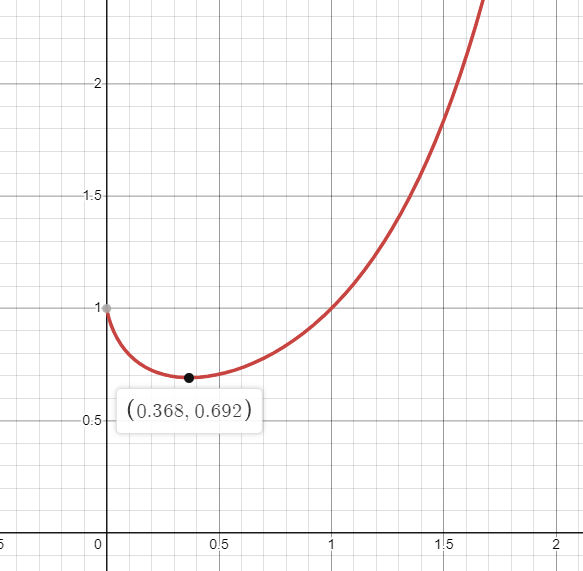
\includegraphics[scale=0.45]{imgs/xxgraph.png}
\end{center}

\subsection{Asymptotes}
An \textbf{inflection point} is the point of the function where it switches concavity.\\
\textbf{Asymptotes} are imaginary lines that are approached by a curve of the graph but never \textit{touch} the curve. 
To find the asymptotes of a function, we compare the numerators and denominators and figure out some information about the function.
\subsubsection{Horizontal Asymptotes}
If the numerator and denominator have the same degree, divide the coefficients by the largest term to get the horizontal asymptote.\\
If the numerator is less than the denominator, then the asymptote is $y = 0$.\\
If the numerator is greater than the denominator, then there is no horizontal asymptote.\\
\\
For example, take $f(x) = \frac{3x^2 + 6x}{x^2 + x}$. The numerator and denominator are both of degree $2$, so we take the quotient of the leading coefficients.\\
$\frac{3}{1} = 3$, so there is a H.A. at $y = 3$.

\subsubsection{Vertical Asymptotes}
Simplify the function, and then find the zeroes of the denominator of the function to determine the vertical asymptotes of the function.\\
\\
For example, for $f(x) = \frac{3x^2 + 6x}{x^2 + x}$, we can simplify the denominator to be $x(x + 1)$, and get a hole at $x = 0$, and a vertical asymptote at $x = 1$.

\subsubsection{Oblique Asymptotes}
Oblique asymptotes use a $y = mx + b$ formula. They are found by dividing its nnumerator by the denominator. The quotient of the division is the equation of the slant asymptote.\\
\\
For example, the oblique asymptote of $y = \frac{3x^3 - 1}{x^2 + 2x}$, by dividing, is $ y = 3x - 6$.

\section{Introduction to Integrals}
\subsection{Summation}
Sigma notation, or summations, take an index starting at $i$ to $n$ and calculate the sum of the function. It is denoted as: $$\sum_{i=0}^{n}$$
For example: $\sum_{i=2}^{4}(2i + 1) = (2\cdot 2 + 1) + (2\cdot3 + 1) + (2\cdot 4 + 1) = 21$\\

\subsubsection{Simplifying Summations}
We can rewrite sums and cancel certain terms out to simplify them. For example:
\begin{enumerate}
    \item $\sum_{i=1}^{100}\tan i - \sum_{i=1}^{50}\tan i = \sum_{i = 51}^{100} \tan i$
    \item $\sum_{i=1}^{N}(2i-1)^5 = \sum_{i=0}^{N-1} (2i+1)^5 = 1^5 + 3^5 + ... + (2N - 1)^5$
    \item $\left[ \sum_{k+1}^{N}x^k \right] + \left[ \sum_{k=0}^{N} k \cdot x^{k+1}\right] = \left[ \sum_{k=2}^{N} k \cdot x^k \right] + N\cdotx^{n + 1} + x$
\end{enumerate}

\subsubsection{Telescope Summation}
Compute the exact value of:
$$\sum_{i=1}^{137} \left[ \frac{1}{i} - \frac{1}{i + 1}\right]$$
We can write the first few terms:
$$(\frac{1}{1} - \frac{1}{2}) + (\frac{1}{2} - \frac{1}{3}) + (\frac{1}{3} - \frac{1}{4}) + ... + (\frac{1}{137} - \frac{1}{138})$$
We see that all the values cancel out, so we're left with $\frac{1}{1}$ and $\frac{1}{138}$, so we have:
$$\sum_{i=1}^{137} \left[ \frac{1}{i} - \frac{1}{i + 1}\right] = 1 - \frac{1}{138} = \frac{137}{138}$$
This series is called a \textbf{telescoping series}, since part of each term gets cancelled by a later term, which then collapses to just 2 terms.

\subsubsection{Partial Fractions and Summations}
Compute the exact value of:
$$\sum_{i=1}^{10,000} \frac{1}{i(i+1)}$$
We note that:
$$\frac{1}{i(i+1)} = \frac{A}{i} + \frac{B}{i+1} = \frac{A(i+1) + Bi}{i(i+1)}$$
Knowing this, we have $i = -1, -B = 1, i = 0, A = 1$.\\
Hence, we get:
$$\sum_{i=1}^{10,000} \frac{1}{i(i+1)} = \sum_{i=1}^{10,000} \left[ \frac{1}{i} - \frac{1}{i + 1}\right]$$

\subsection{Suprema and Infima}
\textbf{Supremum -} The lowest upper bound of a subset. It is always greater than or equal to the maximum of the subset.\\
Equivalently, for $S$ being an upper bound of set $A$:
\begin{enumerate}
    \item If $R$ is an upper bound of $A$, then $S \leq R$.
    \item $\forall R < S, \exists x \in A : R < x < S$.
    \item $\forall \epsilon > 0, \exists x \in A : S - \epsilon < x \leq S$
\end{enumerate}\\
\textbf{Infimum -} The greatest lower bound of a subset. It is always less than or equal to the minimum of the subset.\\
Equivalently, for $L$ being a lower bound on set $A$:
\begin{enumerate}
    \item If $P$ is a lower bound of $A$, then $I \geq P$.
    \item $\forall P > I, \exists x \in A : P > x > L$.
    \item $\forall \epsilon > 0, \exists x \in A : I - \epsilon > x \geq P$
\end{enumerate}

\subsubsection{Consequences of Infima/Suprema}
\begin{enumerate}
    \item $\sup(f+g) < \sup(f) + \sup(g)$
    \item $\sup(f)$ on $[a,c] \geq \max\{\sup(f)$ on $[a,b], \sup(f)$ on $[b,c]\}$
    \item $\sup(cf) \neq c(\sup(f))$
\end{enumerate}
\subsection{Partitions}
A set $P = \{x_1, x_2, ..., x_n\}$ is a partition of $[a,b]$ if:
\begin{enumerate}
    \item $P$ is finite
    \item $x_1 = a, x_n = b$
    \item $P \subset [a,b] \neq \emptyset$\\
    Note that we know $a < x_1 < ... < b$, so it is a strict relation.
\end{enumerate}

\subsubsection{Lower and Upper Sums}
Suppose we had a function $f$. We can determine its area by taking the partition of its intervals.\\
We then take the lower sum $(L_P(f))$ and upper sums $(U_P(f))$ by looking at the minimums and maximums of each interval. Note that $L_P(f)) \leq$ actual area $\leq U_P(f))$\\
The shorter the intervals are between each point in a partition, the more accurate the upper and lower sums become to being the actual area.

\subsubsection{Joining Partitions}
Assume $P, Q$ are two partitions of $[a,b]$.\\
We can take the union of these two partitions, and get a better refinement for the interval $[a,b]$ that can be used to take the integral.\\
In other words, the upper rectangles above $P \cup Q$ are contained in the bigger of the two rectangles from $U_{P}(f)$ and $U_Q(f)$ (similar for the lower rectangles).

\subsubsection{Partitions at Different Intervals}
Let $a < b < c$.
\begin{enumerate}
    \item If $P, Q$ partitions of $[a,b]$, then $P \cup Q$ is a partition of $[a,b]$.
    \item If $P,Q$ partitions of $[a,b]$, then $P \cap Q$ is a partition of $[a,b]$.
    \item If $P$ is a partition of $[a,b]$ and $Q$ is a partition of $[b,c]$, then $P \cup Q$ is a partition of $[a,c]$.
\end{enumerate}

\subsection{Epsilon Definition of Integrals}
Let $f$ be a bounded function on $[a,b]$.\\
If $f$ is integrable on $[a,b]$, then $\forall \epsilon > 0, \exists$ partition of $P$ of $[a,b]$ such that $U_P(f) - L_P(f) < \epsilon$\\
\\
From this, we also know that:
\begin{enumerate}
    \item There exists a partition $P_1$ s.t. $U_{P_1}(f) < I + \frac{\epsilon}{2}$,\\
    since $I + \frac{\epsilon}{2} > I = \inf(U_P(f))$
    \item There exists partition $P_2$ s.t. $L_{P_2}(f) > I - \frac{\epsilon}{2}$.
    \item $U_{P_1}(f) - L_{P_2}(f) < \epsilon$,\\
    since $P = P_1 \cup P_2$
\end{enumerate}

\section{Calculating Integrals}
\subsection{Jump-Discontinued Functions}
Let $f(x) = \begin{cases}
0 & x = 0\\
5 & 0 \leq x \leq 1
\end{cases}$
defined on $[0,1]$.
\begin{enumerate}
    \item Let $P = \{0, 0.2, 0.5, 0.9, 0.1\}$.\\
    Calculate $L_P(f)$ and $U_P(f)$ for this partition.\\
    Since only $f(0) = 0$, every value is the same except for one point where $L_P(f)$ has an area of $5 \cdot 0.2$ at one point.
    
    \item When we fix an arbitrary partition $\{x_0, x_1, ..., x_N\}$ of $[0,1]$. Then, $L_P(f)$ would be the same as $U_P(f)$ for all points except for the area for $5(x_1 - x_0)$.
    
    \item Find a partition $P$ with exactly 3 points (2 subintervals) such that $L_P(f) = 4.99$.\\
    Let $P = \{0, 1- \frac{4.99}{5}, 1\}\}$\\
    $(1 - (1 - \frac{4.99}{5}) = \frac{4.99}{5}$, which we multiply by $5$ to get $4.99$.
    
    \item The upper and lower integrals are both $5$ (since for a single point, it still approaches the same area), therefore $f$ is integrable.
\end{enumerate}
Any function with a single discontinuity will still be integrable since the area can still be calculated.

\subsection{Non-Continuous Functions}
\subsubsection{Theorem on Irrationals/Rationals}
Theorem. Between every two irrational numbers is a rational number.\\
Similarly, between every two rational numbers is an irrational number.

\subsubsection{Calculating the Integral}
Let $f(x) = \begin{cases}
1/2 & 0 \leq x \leq 1/2\\
1 & 1/2 < x \leq 1 \land x \in \mathbb{Q}\\
0 & 1/2 < x \leq 1 \land x \not\in \mathbb{Q}
\end{cases}$
be defined on $[0,1]$.
\begin{enumerate}
    \item Let $P = \{0,0.2, 0.4,0.6,0.8,1\}$. Calculate $L_P(f), U_P(f)$.\\
    Then, we have $L = (0.2)(\frac{1}{2}) + (0.2)(\frac{1}{2}) + 0 + 0 + 0 = 0.2$, and\\
    $U = (0.2)(\frac{1}{2}) + (0.2)(\frac{1}{2}) + 0.2(1) + 0.2 + 0.2 = 0.8$.
    
    \item We can construct a partition $P$ such that $L_P(f) = \frac{1}{4}$ and $U_P(f) = \frac{3}{4}$, where the area at $[0, \frac{1}{2}]$ is $\frac{1}{4}$, and the area at $[\frac{1}{2}, 1]$ is $\frac{1}{2}$
    
    \item The upper integral is equal to $\frac{3}{4}$, and the lower integral is $\frac{1}{4}$.\\
    Since the $\sup$ of the lower sums is not equal to the $\inf$ of upper sums, it is not integrable.
\end{enumerate}

\subsection{Sum of Non-Integrable Functions}
We can find a bounded function $f, g$ on $[0,1]$ such that
\begin{enumerate}
    \item $f$ non-integrable on $[0,1]$,
    \item $g$ non-integrable on $[0,1]$,
    \item $f + g$ integrable on $[0,1]$.
\end{enumerate}
Let $f = \begin{cases}
0 & x \in \mathbb{Q}\\
1 & x \not\in \mathbb{Q}
\end{cases}$,
and let $g = \begin{cases}
1 & x \not\in \mathbb{Q}\\
0 & x \in \mathbb{Q}
\end{cases}$\\
Then the integral of $f + g = 1$.

\subsection{Properties of Integrals}
Let $$\int_{0}^{2} f(x)dx = 3,  \int_{0}^{4}f(x)dx = 9,  \int_{0}^{4}g(x)dx=2$$
We can compute:
\begin{enumerate}
    \item $\int_{0}^{2}f(t)dx = 2f(t)$ (since it is constant respect to $x$).
    \item $\int_{2}^{0}f(x)dx = -3$
    \item $\int_{2}^{4}f(x)dx = \int_{0}^{4}f(x)dx -\int_{0}^{2} f(x)dx = 9 - 3 = 6$
    \item $\int_{-2}^{0}f(x)dx $ cannot be computed.
    \item $\int_{0}^{4}[f(x) - 2g(x)]dx = 9 - 2(2) = 5$.
\end{enumerate}

\subsection{Integrals and Riemann Sums}
The summation of an integral $\sum_{i=1}^n f(\epsilon_i)(\delta_x - \delta_{x-1})$ is considered the Riemann sum.\\
When we take the limit of the Riemann sum as the norm of the partition $||P||$ approaches zero, we can determine the actual area of the function:
$$A = \lim_{||P|| \to 0} \sum_{i=1}^{n} f(\epsilon_i)(\delta_x - \delta_{x-1})$$
which is also the definite integral.

\subsubsection{Riemann Sums Backwards}
Interpret the following limits as integrals.
\begin{align*} 
1. \lim_{n \to \infty}\sum_{i=1}^{n}  \frac{1}{n}\sin(\frac{i}{n}) & & 2. \lim_{n \to \infty}\sum_{i=1}^{n} \frac{n + 1}{n^2} 
\end{align*}
We let $f$ be a continuous function on $[0,1]$. We can write a formula $\int_{0}^{1}f(x)dx$ as a limit of Riemann sums, making the simplest choices you can.\\
Let $n$ be the number of rectangles, and let $i$ be the amount of the rectangle.
So, we have:
$$\lim_{n\to\inty} \sum_{i=1}^{n}(\frac{b-a}{n}) \cdot f(a + i(\frac{b-a}{n}))$$
where $\frac{b-a}{n}$ is the width of the rectangle (length of each subinterval), and $f(a + i(\frac{b-a}{n})$ is the length of each rectangle.\\
\\
Now, we can compute the following limits:
\begin{enumerate}
    \item $\lim_{n \to \infty}\sum_{i=1}^{n}  \frac{1}{n}\sin(\frac{i}{n})$
    \begin{align*}
        \lim_{n \to \infty}\sum_{i=1}^{n}  \frac{1}{n}\sin(\frac{i}{n}) &\\
        & = \int_a^{a+1} f(x) dx\\
        & = \int_0^1 \sin(x) dx
    \end{align*}
    
    \item
    \begin{align*}
        \lim_{n\to\infty}\sum_{i=1}^{n}\frac{n+i}{n^2} & = \lim_{n\to\infty}\sum_{i=1}^{n} (\frac{1}{n})(\frac{n+1}{n})\\
        & = \lim_{n\to\infty}\sum_{i=1}^n(\frac{1}{n})(1+\frac{i}{n})\\
        & = \int_1^2 x dx\\
        & = 1.5
    \end{align*}
    Note that:
    $$\int_a^b f(x)dx = \lim_{n\to \infty} \sum_{i=1}^n (\frac{b-a}{n})f(x_i)$$
    and:
    $$x_i = a + i(\frac{b-a}{n})$$
\end{enumerate}

\subsection{MVT and Integrals}
Theorem. Let $a < b$. Let $f$ be a continuous function on $[a,b]$. There exists $c \in [a,b]$ such that:
$$f(c) = \frac{1}{b-a}\int_{a}^{b}f(t)dt$$
\begin{proof}
    We want to show there exists $c \in [a,b] s.t. f(c) = \frac{1}{b-a} \int_a^bf(x)dx$ on $[a,b]$
    Since $f$ is continuous on $[a,b]$, which is a closed bounded interval, EVT says there exists $c_1 \in [a,b]$ such that $f(c_1)$ is the minimum value of $[a,b]$, and there exists a maximum $f(c_2)$ where $c_2 \in [a,b]$.\\
    The lower sum for $f$ on $[a,b]$ using $P = \{a,b\}$ is $(b-a)(f(c_1))$, where $f(c_1)$ is the minimum value of $f$ on $[a,b]$.\\
    The upper sum for $f$ on $[a,b]$ using $P$ is $b-a(f(c_2))$.\\\\
    We know continuous functions are integrable, so $f$ is integrable. We then know by integrable that $L \leq \int_a^bf \leq U$.\\
    We can divide everything by $(b-a)$ to get:
    $$f(c_1) \leq \frac{1}{b-a} \int_a^bf \leq f(c_2)$$
    Since $f$ continuous, IVT says there exists a $c$ such that $a < c < b$, where $f(c) = \frac{1}{b-a} \int_a^b f$.
\end{proof}

\subsection{Initial Value Problem}
Find a function $f$ such that:
\begin{enumerate}
    \item $\forall x \in \mathbb{R}, f''(x) = \sin(x) + x^2$,
    \item $f'(0) = 5$,
    \item $f(0) = 7$
\end{enumerate}
Looking at $f''$, we know $f'(x) = -\cos x + \frac{x^3}{3} + 6$.\\
Then, $f(x) = -\sin(x) + \frac{x^4}{12} + 6x + 7$

\subsection{Computing Antiderivatives}
\begin{enumerate}
    \item $\int x^5 dx = \frac{x^6}{6}$
    \item $\int (3x^8 - 18x^5 + 1) dx = \frac{x^9}{3} - 3x^6 + x + C$
    \item $\int \sqrt[3]{x}dx = \int x^{\frac{1}{3}}dx = \frac{3}{4}x^{\frac{4}{3}} + C$
    \item $\int \frac{1}{x^9}dx = \int x^{-9} dx = \frac{x^{-8}}{-8} + C$ 
\end{enumerate}

\subsection{Completing the Squares}
Sometimes, it is easier to use squares to compute values of functions.\\
\\
Example: Complete the square for $2x^2 + 12x + 1$.
\begin{align*}
    2(x^2 + 6x + A - A) + 1\\
    2(x+A)(x+A) - B +1
\end{align*}
To get a square with a term 6x, we can let $A=3$. Then:
\begin{align*}
    2(x+3)(x+3) - 18 + 1 & = 2(x+3)^2 - 17
\end{align*}
So, we have $2(x^2+6x+9-9)+1$.

\section{Fundamental Theorem of Calculus}
Let $F'(x) = f(x)$ (that is, $F(x)$ is the antiderivative of $f(x)$). Then:
$$\int_a^b f(x) dx = F(b) - F(a)$$
We utilize the following terms:
\begin{enumerate}
    \item \textbf{Antiderivatives} of $f(x)$ is a function with derivative equal to $f(x)$.
    \item \textbf{Definite Integrals} are defined as $\int_a^b f(x)dx = \left[ F(x) \right]_a^b = F(b) - F(a)$.\\
    It is the net area between $f$ and the x-axis on $[a,b]$ AND the total change in the antiderivative (e.g., integral of velocity = total change in position/displacement).
    \item \textbf{Indefinite Integrals} are defined as $\int f(x)dx = F(x) + C$.\\
    It is the integral defined when there is no upper and lower limit.
\end{enumerate}

\subsection{Graphing Functions Using FTC}
Suppose we have a graph $F(x) = \int_0^x f(t) dt$. We want to graph $f(t)$.
\begin{enumerate}
    \item Calculate some exact values of $f$ using FTC, i.e., $f(1) - f(0) = \int_0^1 F(x)$.
    \item Check when $f$ is increasing, i.e., when $F(x) > 0$.\\
    Going from decreasing to increasing implies there is a minimum. Going from increasing to deccreasing implies there is a maximum.\\
    Note that integrating from right to left switches the sign of the width.
\end{enumerate}

\subsection{Some Statements on Integrals}
\begin{enumerate}
    \item Let $f(x) = \int_0^x g(t) dt$. Can an anti-derivative of $g(x) $ be written as $\int_0^x g(t)dt$?\\
    We have $\frac{d}{dx} \left[ \int_0^x g(t) dt \right] = f'(x) = g(x)$. Since the derivatives are equal, the functions are equal except for maybe a constant.\\
    Note that $f(x) = \int_0^x g(t) dt$ is not true for all anti-derivatives of $g$; just one of them. We use the extra quantifier/constant but it does not always make the statement true.
    
    \item If $f(0) = 0$, then $f(x) = \int_0^x g(t) dt$.\\
    We can interpret this as ``If an anti-derivative of $g$ is 0 at $x = 0$, then it can be written as $\int_0^x g(t) dt$''\\
    Note that there is no extra quantifier on $f$ to make this true.
    
    \item There exists a $C \in \mathbb{R}$ such that $f(x) = C + \int_0^x g(t) dt$. We can set $C$ to just be equal to the integral to make the two values equal.
\end{enumerate}

\subsection{Calculating Derivatives Using FTC}
Find $\frac{d}{dx} F(x)$ for the following integrals:
\begin{enumerate}
    \item $F(x) = \int_0^1 e^{-x^2} dt$
    \begin{align*}
        \frac{d}{dx} F(x) & = \frac{d}{dx} [\text{constant}]\\
        & = 0
    \end{align*}
    
    \item $F(x) = \int_0^x e^{-\sin(t)} dt$
    \begin{align*}
        \frac{d}{dx} F(x) & = \frac{d}{dx}[F(x) - F(0)]\\
        & = F'(x) - 0 & \text{Where } F' = e^{-\sin(t)}\\
        & = e^{-\sin(t)}
    \end{align*}
    
    \item $F(x) = \int_1^{x^2} \frac{\sin t}{t^2} dt$
    \begin{align*}
        \frac{d}{dx} F(x) & = \frac{d}{dx} G(x^2)\\
        & = G'(x^2) \cdot (2x)\\
        & = \frac{\sin(x^2)}{(x^2)^2} \cdot (2x) & \text{since } \int_1^x \frac{\sin t}{t^2} dt \implies G'(x) = \frac{\sin(x)}{x^2}
    \end{align*}
    
    \item $F(x) = \int_x^7 \sin^3(\sqrt{t}) dt$
    \begin{align*}
        \int_x^7 \sin^3(\sqrt{t}) dt & = - \int_7^x \sin^3(\sqrt{t}) dt\\
        \frac{d}{dx} \left( \int_x^7 \sin^3(\sqrt{t}) dt \right) & = \frac{d}{dx} \left( - \int_7^x \sin^3(\sqrt{t}) dt \right)\\
        & = -\sin^3(\sqrt{x})
    \end{align*}
    
    \item $F(x) = \int_{2x}^{x^2} \frac{1}{1 + t^3} dt$
    \begin{align*}
        \int_{2x}^{x^2} \frac{1}{1 + t^3} dt & = \frac{d}{dx} \left[ \int_0^{x^2} \frac{1}{1 + t^3} dt - \int_0^{2x} \frac{1}{1 + t^3} dt \right]\\
        & = \frac{1}{1 + (x^2)^3} \cdot (2x) - \frac{1}{1 + (2x)^3} \cdot 2
    \end{align*}
\end{enumerate}

\subsection{Generalizing FTC}
Let $f, u, v$ be differentiable functions with domain $\mathbb{R}$. We define:
$$F(x) = \int_{u(v)}^{v(x)} f(t) dt$$
Find a formula for $F'(x)$.
\begin{align*}
    F(x) & = \int_0^{v(x)} f(t) dt - \int_0^{u(x)} f(t) dt\\
    \frac{d}{dx} F(x) & = f(v(x)) \cdot v'(x) - f(u(x)) \cdot u'(x)
\end{align*}

\subsection{Integrals With Substition}
Suppose we have $\left[ f(g(x)) \right]'$. Using chain rule, we have it equal to $f'(g(x)) \cdot g'(x)$. So, when we take the integral, we can substitute $g(x)$ as a variable to simplify our calculations: 
\begin{align*}
    \int f'(g(x)) \cdot g'(x) dx & = \int f'(w) dw & \text{Where } w = g(x), \ \ \frac{dw}{dx} = g'(x), \ \ dw = g'(x) dx\\
    & = f(w) + c\\
    & = f(g(x)) + c
\end{align*}

\subsubsection{Examples Using Substitution}
\begin{enumerate}
    \item $\int (3x^2 + 4)\sqrt{x^3 + 4x - 1} dx$\\
    Let $w = x^3 + 4x - 1$, $\frac{dw}{dx} = (3x^2 + 4)$, $dw = (3x^2 + 4) dx$
    \begin{align*}
    \int (3x^2 + 4)\sqrt{x^3 + 4x - 1} dx & = \int \sqrt{w} dw\\
    & = \int w^{\frac{1}{2}} dw\\
    & = \frac{2}{3} w^{\frac{3}{2}} + c\\
    & = \frac{2}{3}(x^3 + 4x - 1)^{\frac{3}{2}} + c
    \end{align*}
    
    \item $\int_{\frac{1}{2}}^{\frac{1}{\sqrt{2}}} \frac{4}{\sqrt{1 - x^2}} dx$\\
    Let $x = \sin(w)$, and $\dx = \cos(w) dw$. Note that $\arcsin(\sin w) = \arcsin x$, and $[\frac{1}{2}, \frac{1}{\sqrt{2}}]$ are in the domain where $\arcsin(\sin(\theta)) = \theta$
    \begin{align*}
        \int_{1/2}^{1/\sqrt{2}}\frac{4}{\sqrt{1-x^2}}dx & = \int_?^? \frac{4 \cos(w)}{\sqrt{1-\sin^2w}}dw\\
        & = \int_?^? \frac{4\cos w}{\cos^2w}dw\\
        & = \int_?^? 4 dw\\
        & = [4w]_?^?\\
        & = [4 \arcsin(x)]_{1/2}^{1/\sqrt{2}} & \text{Since }\frac{d}{dx}\arcsin(x) = \frac{1}{\sqrt{1-x^2}}\\
        & = 4\arcsin(\frac{1}{\sqrt{2}})\\
        & = \frac{4\pi}{4} - \frac{4\pi}{6}\\
        & = \frac{\pi}{3}
    \end{align*}
\end{enumerate}

\subsection{Computing Definite Integrals}
\begin{enumerate}
    \item $\int_1^2 x^3 dx$
    \begin{align*}
        \int_1^2 x^3 dx & = \left[ \frac{x^4}{4} \right]_1^2\\
        & = \frac{2^4}{4} - \frac{1^4}{4} = 4 - \frac{1}{4} = \frac{15}{4}
    \end{align*}
    
    \item $\int_0^1 \left[ e^x + e^{-x} - \cos(2x)\right] dx$
    \begin{align*}
        \int_0^1 \left[ e^x + e^{-x} - \cos(2x)\right] dx & = \left[ e^x - e^{-x} - \frac{\sin(2x)}{2}\right]_0^1\\
        & = \left[ e^1 - e^{-1} - \frac{\sin 2}{2}\right] - \left[ e^0 - e^{-0} - \frac{\sin(0)}{2}\right]\\
        & = (e - \frac{1}{e} - \frac{\sin 2}{2}) - (1 - 1 - 0)\\
        & = e - \frac{1}{e} - \frac{\sin 2}{2}
    \end{align*}
    
    \item $\int_{\pi/4}^{\pi/3}\sec^2x dx$
    \begin{align*}
        \int_{\pi/4}^{\pi/3}\sec^2x dx & = [\tan(x)]_{\pi/4}^{\pi/3}\\
        & = \tan\frac{\pi}{3} - \tan\frac{\pi}{4}\\
        & = \frac{\sqrt{3}}{2} - 1
    \end{align*}
    
    \item $\int_1^2 \left[\frac{d}{dx}(\frac{\sin^2x}{1 + arctan^2x + e^{-x^2}})\right]$
    \begin{align*}
        \int_1^2 \left[\frac{d}{dx}(\frac{\sin^2x}{1 + arctan^2x + e^{-x^2}})\right] & = \frac{\sin^2(2)}{1 + \arctan^2(2)+e^{-4}} - \frac{\sin^2(1)}{1 + \arctan^2(1) + e^{-1}}
    \end{align*}
\end{enumerate}


\subsubsection{Aside About Circles}
The collection of points $(x,y)$ that are one unit away from $(0,0)$ is:
$$1 = \sqrt{(x-0)^2 + (y-0)^2}$$
$$1 = x^2 + y^2 \implies y = \pm \sqrt{1-x^2}$$


\subsection{Areas Using Integrals}
When we calculate the areas under curves of a function, it can be zero or negative. However, we mostly deal with signed areas of the function which deal with negative and positive values of the graph.\\
If we want the total unsigned area, we can use absolute values, instead.

\subsubsection{Examples}
\begin{enumerate}
    \item Write the integral between $y = \cos(x)$, the $x-$axis, from $[0,\pi]$.\\
    We know $\cos(x)$ is positive on $[0,\pi/2]$ and negative from $[\pi/2,\pi]$. So, our unsigned area is:
    $$|\int_0^{\pi/2} \cos(x) dx| + \int_{\pi/2}^{\pi}\cos(x) dx$$
    
    \item Write the integral between $y=x^2+3$ and $y=3x+1$.\\
    First, find the intersection points:
    \begin{align*}
        x^2 + 3 & = 3x + 1\\
        x^2 - 3x + 2 & = 0\\
        (x-1)(x-2) & = 0
    \end{align*}
    So, our intersection points are $x = 1, x=2$. Next, we can calculate the integral.
    $$\int_1^2 (3x+1) - (x^2+3) dx = \int_1^2 (3x-2-x^2)dx$$
\end{enumerate}

\subsubsection{Minimizing Area}
For the function
$$f_a(x) = (1+a) - ax^2$$
find the value of $a >0$ that minimizes the area of the region bounded by the graph of $f_a$ and the $x-$axis.\\
First, we set up the integral:
$$\int 1 + a - ax^2 dx$$
We want to find the endpoints of $x$, so we use the quadratic formula:
$$x_i = \frac{0\pm \sqrt{-4(1+a)a}}{-2a}$$
Using this endpoint, we then can find this area (multiplying by 2 since it is symmetric above the $y-$axis:
$$2 \int_0^{x_i} 1 + a - ax^2 dx$$

\subsubsection{Finding Length From the Area}
What is the length of the rectangle with a a base $[a,b]$, and the area $\int_a^b f(x)dx$?\\
Using the area of a rectangle we know that:
$$(b-a)(l) = \int_a^b f(x)dx$$
So, we can say that the length of the rectangle is:
$$l = \frac{1}{b-a}\int_a^b f(x)dx$$
This is equivalent to the \textbf{average value of a function}.

\section{Integration Techniques}
\subsection{Simplification and Guess-and-Check}
Simplification can be used to help make equations easier to compute and understand.\\
\\
Example 1:
\begin{align*}
    \int (x^2 + 6)^2 dx & = (x^2 + 6)(x^2 + 6) dx\\
    & = (x^4 + 12x^2 + 36) dx
\end{align*}
Check: $\frac{d}{dx} x^5 = 5x^4$. So, $\frac{d}{dx} \frac{x^5}{5} = \frac{1}{\not 5}\not 5 x^4$.\\
Then, $\frac{d}{dx} 4x^3 = 12x^2$. Hence:
\begin{align*}
    (x^4 + 12x^2 + 36) dx & = \frac{x^5}{5} + 4x^3 + 36x + c
\end{align*}

\subsection{Integration By Substitution}
For an integral $\int f'(g(x))g'(x) dx$, we can let $w = g(x)$, then $dw = g'(x) dx$.
\begin{align*}
    \int \frac{5x + 3}{\sqrt{\frac{5}{2}x^2 - 3x - 1}} dx & = \int \frac{dw}{\sqrt{w}} & \text{Since } w = \frac{5}{2}x^2 - 3x - 1, \ \ dw = (5x+3) dx\\
    & = \int w^{-1/2}dw\\
    & = 2w^{1/2} + c\\
    & = 2\sqrt{\frac{5}{2} x^2 + 3x - 1} + c & \text{Since }\frac{d}{dw} w^{1/2} = \frac{1}{2}w^{-1/2}
\end{align*}

\subsubsection{Examples}
\begin{enumerate}
    \item $\int \frac{\sin(x^{1/2}}{x^{1/2}}$\\
    Let $w = x^{1/2} dx$. Then $2dw = \frac{2}{2\sqrt{x}} dx$.
    \begin{align*}
        \int \frac{\sin(x^{1/2}}{x^{1/2}} & = \int 2 \sin(w) dw\\
        & = -2 \cos(w) + c\\
        & = -2 \cos(\sqrt{x}) + c
    \end{align*}
    
    \item $\int e^x \cos(e^x) dx$\\
    Let $w = e^x, dw = e^x dx$.
    \begin{align*}
        \int e^x \cos(e^x) dx & = \int \cos(e^x) \cdot (e^x dx)\\
        & = \int \cos(w) dw\\
        & = \sin(w) + c\\
        & = \sin(e^x) + c
    \end{align*}
    
    \item $\int \cot(x) dx = \int \frac{\cos(x)}{\sin(x)} dx$\\
    Let $w = \sin(x), dw = \cos(x) dx$.
    \begin{align*}
        \int \frac{\cos(x)}{\sin(x)} dx & = \int \frac{dw}{w}\\
        & = \int \frac{1}{w}\\
        & = \ln|w| +c\\
        & = \ln|\sin(x)| +c
    \end{align*}
    
    \item $\int x^2\sqrt{x + 1} dx$
    Let $w = \sqrt{x + 1} = (x+1)^{1/2}$. Then, $dw = \frac{1}{2}(x+1)^{-1/2} dx = \frac{1}{2\sqrt{x+1}} dx = \frac{1}{2w} dx$. Hence $2wdw = dx$.\\
    Then, $w^2 = x + 1$, $x = w^2 -1$, $x^2 = (w^2 -1)^2$. So:
    \begin{align*}
        \int x^2\sqrt{x + 1} dx & = \int (w^2-1)^2 2w^2 \ dw\\
        & = \int (w^4 - 2w^2 - 1)2w^2 dw\\
        & = \int 2w^6 -4w^4 - 2w^2 dw\\
        & = \frac{2}{7}w^7 - \frac{4}{5}w^5 - \frac{2}{3}w^3 + c\\
        & = \frac{2}{7}(x+1)^{7/2} - \frac{4}{5}(x+1)^{5/2} - \frac{2}{3}(x+1)^{3/2} + c
    \end{align*}

    \item $\int \frac{e^2x}{\sqrt{e^x +1}}$\\
    Let $w = e^x, dw = e^x dx$.
    \begin{align*}
        \int \frac{e^2x}{\sqrt{e^x +1}} & = \int \frac{e^x \cdot e^x}{\sqrt{e^x + 1}} dx\\
        & = \int \frac{w}{\sqrt{w + 1}} dw\\
        & = \int \frac{z-1}{\sqrt{z}} dw & \text{Let }z = w+1, \ \ z - 1 = w, \ \ dz = dw\\
        & = \int \frac{z}{z^{1/2}} - z^{-1/2} dz\\
        & = \int z^{1/2} - z^{-1/2} dz\\
        & = \frac{2}{3}z^{3/2} - 2z^{1/2} + c\\
        & = \frac{2}{3}(e^x+1)^{3/2} - 2(e^x + 1)^{1/2} + c
    \end{align*}
    
    \item $\int \frac{\ln(\ln(x))^2}{x \ln x} dx$\\
    Let $w = \ln(x), dw = \frac{1}{x} dx$.
    \begin{align*}
        \int \frac{\ln(\ln(x))^2}{x \ln x} dx & = \int \frac{(\ln(w))^2}{w} dw\\
        & = z^2dz & \text{Let }z = \ln(w), dz = \frac{1}{w} dw\\
        & = \frac{z^3}{3} + c\\
        & = \frac{(\ln(w))^3}{3} + c\\
        & = \frac{[\ln(\ln(x)]^3}{3} + c
    \end{align*}
    
    \item $\int x e^{-x^2} dx$\\
    Let $w = -x^2$, and $\frac{dw}{-2} = \frac{\not{-2}x}{\not{-2}} dx$.
    \begin{align*}
        \int x e^{-x^2} dx & = e^w dw\\
        & = e^w + c\\
        & = e^{-x^2} + c
    \end{align*}
    
    \item $\int_0^2 \sqrt{x^3 +1} x^2 dx$\\
    Let $w = x^3 + 1$, and $\frac{dw}{3} = \frac{\not{3}x^2}{\not 3} dx$
    Method 1:
    \begin{align*}
        \int_0^2 \sqrt{x^3 +1} x^2 dx & = \int_?^? \frac{\sqrt{w}}{3} dw\\
        & = \left[ 3\frac{2w^{3/2}}{3}\right]_?^?\\
        & = \left[ 2(x^3+1)^{3/2} \right]_0^2\\
        & = 2(9^{3/2}) - 2
    \end{align*}
    Method 2:\\
    If $x: 0 \to 2$, then $w: 0^3 + 1 \to 2^3 + 1$
    \begin{align*}
        \int_0^2 \sqrt{x^3 +1} x^2 dx & = \int_1^9 \frac{\sqrt{3}}{3}dw\\
        & = \left[ 2w^{3/2}\right]_1^9\\
        & = 2(9)^{3/2} - 2(1)^{3/2}
    \end{align*}
\end{enumerate}

\subsection{Integration By Parts}
For a derivative, we have $(f \cdot g)' = f'g + fg'$. Similarly for integrals:
\begin{align*}
    \int (f(x)g(x))' dx & = \int f'(x)g(x) dx + \int f(x)g'(x) dx\\
    f(x)g(x) & = \int f'(x)g(x) dx + \int f(x)g'(x) dx\\
    \int f'(x)g(x) dx & = f(x)g(x) - \int f(x)g'(x) dx
\end{align*}
For example:
\begin{align*}
    \int x \ln(x) dx\\
    \int u \ dv &  = uv - \int v \ du
\end{align*}
We don't know how to integrate $\ln(x)$, so let $u = \ln(x)$, with $dv = x \ dx$. Then, $du = \frac{1}{x} dx$, and $v = \frac{x^2}{2}$. Then:
\begin{align*}
    \int x \ln(x) dx & = \frac{x^2}{2}\ln(x) - \int \frac{x^2}{2} \cdot \frac{1}{x} dx\\
    & = \frac{x^2}{2} \ln(x) - \frac{1}{2} \int x \ dx\\
    & = \frac{x^2}{2} \ln(x) - \frac{1}{2} \cdot \frac{x^2}{2} + c
\end{align*}

\subsubsection{Examples}
\begin{enumerate}
    \item $\int x e^{-2x} dx$\\
    Let $u = x, dv = e^{-2x}dx$. Then, $du = dx, v = \frac{e^{-2x}}{-2}dx$.
    \begin{align*}
        \int x e^{-2x} dx & = x \frac{e^{-2x}}{-2} - \int \frac{e^{-2x}}{-2} dx
    \end{align*}
    We have $\frac{d}{dx}\frac{e^{-2x}}{-2} = e^{-2x}$, and\\
    $\frac{d}{dx} \frac{e^{-2x}}{4} = \frac{1}{4}e^{-2x}(-2)$. So
    \begin{align*}
     x \frac{e^{-2x}}{-2} - \int \frac{e^{-2x}}{-2} dx & = \frac{xe^{-2x}}{-2} - \frac{e^{-2x}}{4} + c
    \end{align*}
    
    \item $\int x^2 \sin x \ dx$\\
    Let $u = x^2, dv = \sin x \ dx$. Then, $du = 2x \ dx, b = -\cos x$.
    \begin{align*}
        \int x^2 \sin x \ dx & = - x^2 \cos(x) + 2 \int x \cos(x) dx
    \end{align*}
    Then, let $u = x, dv = \cos x \ dx$. We also have $du = dx, v = \sin x$.
    \begin{align*}
        - x^2 \cos(x) + 2 \int x \cos(x) dx & = - x^2 \cos x + 2[x \sin(x) - \int \sin x \ dx]\\
        & = -x^2 \cos x + 2x \sin x - 2[-\cos x] + c
    \end{align*}
    
    \item $\int \ln x \ dx$\\
    Let $u = \ln x, dv = dx$. Then, $du = \frac{1}{x} dx, v = x$.
    \begin{align*}
        \int \ln x \ dx & = x \ln x - \int x \frac{1}{x} dx\\
        & = x \ln x - \int 1 dx\\
        & = x \ln x - x + c\\
        & = x(\ln x - 1) + c
    \end{align*}
    
    \item $\int \sin \sqrt{x} dx$\\
    Let $u = \sin \sqrt{x}, dv = dx$. Then, $du = \frac{\cos \sqrt{x}}{2\sqrt{x}}, v = x$.
    \begin{align*}
        \int \sin \sqrt{x} dx & = x \sin \sqrt{x} - \frac{1}{2} \int \frac{x}{\sqrt{x}} \cos \sqrt{x} \ d \sqrt{x}
    \end{align*}
    Then, let $u = \cos{x}, dv = x^{1/2}$, and $du = \frac{- \sin \sqrt{x}}{2 \sqrt{x}}dx, v = \frac{2}{3}x^{3/2}$.
    \begin{align*}
        
    \end{align*}
    
    \item $\int_1^e (\ln(x))^3 dx$\\
    Let $u = (\ln x)^3, dv = dx$, then $du = \frac{3(\ln(x)^2}{x} dx, v = x$.
    \begin{align*}
        \int_1^e (\ln(x))^3 dx & = \left[ x(\ln x)^3\right]_1^3 -3 \int_1^e (\ln x)^2 dx
    \end{align*}
    Let $u = (\ln x)^2, dv = dx$, then $du = \frac{2 \ln x}{x} dx, v = x$.
    \begin{align*}
        & = \left[x (\ln x)^3\right]_1^e - 3 \left[ [x(\ln x)^2]_1^e - 2 \int_1^e \ln x dx \right]
    \end{align*}
    Let $u = \ln x, dv = dx$, then $du = \frac{1}{x} dx, v = x$.
    \begin{align*}
        & = \left[ x (\ln x)^3 \right]_1^e - 3 \left[ x (\ln x)^2 \right]_1^e + 6\left[ [x \ln x]_1^e - \int_1^e dx\right]\\
        & = (e - 0) - 3(e- 0) + 6(e - 0) - [x]_1^e\\
        & = 3e - 1
    \end{align*}
\end{enumerate}
\subsection{Partial Fractions}
The integrals of partial fractions are calculated similarly to rational fractions, however, partial fractions typically have a denominator with a larger degree than the numerator.\\
If the numerator is bigger than the denominator, use division or substitution.
\begin{enumerate}
    \item $\int \frac{1}{(x+1)(x-3)} dx$\\
    Let this be equal to $\int \frac{A}{x+1} + \frac{B}{x-3}dx$. Then:
    \begin{align*}
        \frac{A(x-3) + B(x+1)}{(x+1)(x-3)} & = \frac{1}{(x+1)(x-3)}
    \end{align*}
    So:
    \begin{align*}
        Ax - 3A + Bx + B & = 1\\
        (A+B)x + (B-3A) & = 0x + 1
    \end{align*}
    Hence, we know $A+B = 0$, or $A= -B$, and for our constants we have $B - 3A = 1, B-3(-B) = 1, 4B = 1$. Thus, $B=\frac{1}{4}$. Using this, we have:
    \begin{align*}
        \int \frac{1}{(x+1)(x-3)}dx & = \int \frac{-1/4}{x+1} + \frac{1/4}{x-3} dx\\
        & = \frac{-1}{4} \ln |x+1| + \frac{1}{4} \ln |x-3| + C
    \end{align*}
    
    \item $\int \frac{1}{(x+1)^n} dx$\\
    We can use substitution. Let $w = x+1, dw = dx$.
    \begin{align*}
        \int \frac{1}{(x+1)^n} dx & = \int \frac{1}{w^n} dw\\
        & = \int w^{-n}dw & = \frac{w^{-n+1}}{-n+1} + C\\
        & = \frac{(x+1)^{1-n}}{1-n} +c
    \end{align*}
    
    \item $\int \frac{(x+1)-1}{(x+1)^2}dx$
    We can cancel out the $x+1$ term.
    \begin{align*}
        \int \frac{x+1}{(x+1)^2} - \frac{1}{(x+1)^2} dx\\
        & = \int \frac{1}{x+1} - (x+1)^{-2} dx\\
        & = \ln |x+1| + (x+1)^{-1} + c
    \end{align*}
    \\
    We can do a similar process with partial fractions.
    \begin{align*}
        \int \frac{A}{(x+1)^1} + \frac{B}{(x+1)^2} dx = \frac{A(x+1) +B}{(x+1)^2}  = \frac{x}{(x+1)^2}
    \end{align*}
    So, we have:
    \begin{align*}
        Ax + A + B = x & \iff Ax + (A+B) = 1x + 0 
    \end{align*}
    So, $A = 1, A+B=0$, meaning $A = -B, B = -1$. Then:
    \begin{align*}
    \int \frac{1}{x+1} - \frac{1}{(x+1)^2}dx,
    \end{align*}
    which then is solved the same way as above.
    
    \item $\int\frac{2x+6}{(x+1)^2}dx$\\
    We have:
    \begin{align*}
        \int \frac{A}{x+1} + \frac{B}{(x+1)^2}dx & = \int \frac{A(x+1) +B}{(x+1)^2}dx
    \end{align*}
    So, $2x+6 = Ax + A + B$. Then $2x = Ax \implies 2 = A$, and $6 = A + B \implies B = 4$. Thus:
    \begin{align*}
        \int \frac{2}{x+1} + \frac{4}{(x+1)^2}dx & = 2 \ln|x+1| - 4(x+1)^{-1} +c
    \end{align*}
    
    \item $\int \frac{x^2}{(x+1)^3}dx$\\
    We have $\int \frac{A}{x+1} + \frac{B}{(x+1)^2} + \frac{C}{(x+1)^3}dx$\\
    Let $w = x+1 \implies x = w -1$. Then, $dw = dx$.
    \begin{align*}\
    \int \frac{(w-1)^2}{w^3}dw & =\int \frac{w^2}{w^3} - \frac{2w}{w^3} + \frac{1}{w^3}dw\\
    & = \int \frac{1}{w} - \frac{2}{w^2} + \frac{1}{w^3}dw\\
    & = \ln |w| + 2w^{-1} - \frac{w^{-2}}{2} + c\\
    & = \ln |x+1| + 2(x+1)^{-1} - \frac{(x+1)^{-2}}{2} + c
    \end{align*}
    
    \item $\int \frac{p(x)}{x^4(x+1)^3(x+2)(x^2+1)(x^2+4)}$\\
    We can expand this (make sure to get all terms):
    $$\int \frac{A}{x} + \frac{B}{x^2} + \frac{C}{x^3} + \frac{D}{x^4} + \frac{E}{(x+1)} + \frac{F}{(x+1)^2} + \frac{G}{(x+1)^3} + \frac{H}{(x+2)} + \frac{I}{x^2+1} + \frac{J}{x^2+4} dx$$
\end{enumerate}

\section{Volumes}
For any shape with the same cross-section (e.g., prisms), calculate the area of the face, then multiply it by the distance of the object.\\
More generally, we can say:
$$V = \int_a^b A(x) dx$$

\begin{enumerate}
    \item \textbf{Prisms}\\
    Take a prism with a base defined as $x^2 + y^2 = 5$. with a height of $2$.\\\\
    Generally, we solve volumes by multiplying 2 by the integral of half of the prism. In this case, it is $y = \sqrt{5-x^2}$. Then, we know we go from a height of 0 to 2 for the distance of the prism, so we integrate from 0 to 2.\\
    Hence, our volume is $V = 2 \int_0^2 \sqrt{5 - x^2} dx$
    \item \textbf{Pyramids}\\
    Compute the volume of a pyramid with height $H$ and the square base with side length $L$.\\\\
    Geometrically, we determine this as a square base that gets smaller and smaller as the height of the pyramid increases. If $n$ represents the number of slices, as $n \to \infty,$ the height approaches $dy$.\\
    We can then draw triangles as the cross section of the object, where the base of the triangle is $\frac{1}{2} L$ and the height is $H$. \\
    As the height gets smaller, we get smaller triangles, which are defined as $h = H - y$, and $2l = \frac{(H-y)L}{H}$. $l$ describes half the distance of the cross section (the pyramid's base at height $y$).\\
    Now, we can calculate the volume: $\int_0^H (\frac{(H-y)L}{H})^2 dy$.
    \item \textbf{Other Volumes}\\
    Find the volume of the shape with base bordered by the $x-$axis, $y-$axis, and $y= 6-x$, and has a square cross-section, which is parallel to the $y$-axis.\\\\
    The resulting shape will look something like a wedge (a square base that forms a triangular point).\\
    The cross-section of the square base gets gradually smaller as $x$ increases until $x = 6$ (where the function becomes a zero), so we know we integrate from 0 to 6.\\
    The height of the shape is dependent on the $y$ value as $x \to 6$, so we know we take the value of $y$ at each $x$ value to determine the volume.\\
    Hence:  $V = \int_0^6 = (y)^2 dx = \int_0^6 (6-x)^2 dx$.
\end{enumerate}

\subsection{Volumes of Rotation}
Using volumes of rotation is useful when we want to find the volume of something that started as a two-dimensional area. Usually, we rotate around a certain point (either in the $y$ or $x$ axis) in order to create circles in the third-dimension (or cylinders), of which the volume can then be calculated.\\
You can calculate these volumes using:
\begin{enumerate}
    \item \textbf{Washers} - 2D circles that sometimes have holes in the centre of them.\\
    General Formula: $$\int_a^b (\pi r^2) dx = \int_a^b \pi (f(x))^2 dx$$
    If we rotate around the $y$-axis, we use $\int_a^b \pi (g(y))^2 dy$.\\
    \\
    Example: Volume of a Sphere.\\
    We know the equation of a circle with radius $r$ centred around $(0,0)$ is $x^2 + y^2 = r^2$.\\
    If we rotate the circle around the $x$-axis, we can produce a sphere. We integrate in terms of $y$, so we find the radius $y = \sqrt{r^2 - x^2}$. Hence, we get the integral $\int_{-r}^{r} \pi (\sqrt{r^2 - x^2})^2 dx$. Expanding this we have:
    \begin{align*}
        \int_{-r}^{r} \pi (\sqrt{r^2 - x^2})^2 dx & = \int_{-r}^{r} \pi (r^2 - x^2)dx\\
        & = \pi\left[ r^2x - \frac{x^3}{3}\right]_{-r}^r\\
        & = \pi\left[(r^3 - \frac{r^3}{3}) - (r^2(-r)  - \frac{(-r)^3}{3})\right]\\
        & = \pi\left[ \frac{2}{3}r^3 + \frac{2}{3}r^3\right]\\
        & = \frac{4}{3}\pi r^3
    \end{align*}
    \item \textbf{Cylindrical Shells} - 3D cylinders that sometimes have holes in the centre of them).\\
    General Formula: We calculate the area of the cylinder using the rectangular cross-section of a cylinder (defined as $2\pi r)$, and then multiply this value by the height of the shape.\\
    When we rotate around the $y-$axis, our $x$-values represent a different height of the cylindrical shells. \\
    Hence:
    $$\int_a^b (2\pi r)y dx = \int_a^b 2\pi f(x) \cdot x dx$$\\
    \\
    Example: Determine the volume created by rotating $\Omega$ around the $y-$axis where $\Omega$ is the area bounded between $y=x^5 + x -2$, $x = 2$, and the $x-$axis.\\
    \\
    Here, we know we're integrating from $0$ to $2$ based on our bounds. When rotating around the $y-$axis, we integrate in terms of $x$, so we have the following formula:
    \begin{align*}
        \int_0^2 2\pi x y dx & = \int_0^2 2\pi x(x^5 + x - 2) dx\\
        & = 2\pi \int_0^2(x^6 + x^2 - 2x)dx
    \end{align*}
\end{enumerate}

\subsubsection{More Examples}
Let $\Omega$ be the finite area bounded between $y=x^2$, the $x-$axis, and $x=1$.\\
Find the formulas for the following volumes of rotation:
\begin{enumerate}
    \item Rotating around $y=0$:
    \begin{enumerate}
        \item Washers: Our cross-section becomes circles that become bigger as they get closer to $x=1$. Here, we use the area of a circle $(\pi r^2)$ $r$ is the perpendicular axis of rotation.\\
        Hence, our volume is $\int_0^1 \pi(x^2)^2 dx$.
        \item Cylindrical Shells: We create cylinders that get bigger as they approach $x=1$. We use the surface area of a cylinder, where $r$ is the perpendicular axis of rotation, and $h$ is parallel to the axis of rotation.\\
        Note that $y = x^2$, and so we get $x = 1 - \sqrt{y}$ as our radius.\\
        Hence, our volume is $\int_0^1 2\pi(y)(1-\sqrt{y}) dy$
    \end{enumerate}
    
    \item Rotating around $y=2$:
    \begin{enumerate}
        \item Washers: Here, we have a ``cut-out'' for the volume, so we have the larger circle $\pi(2)^2(1)$, and our smaller cutout (which gets smaller as $x \to 1$).\\
        Hence, our volume is: $\int_0^1 \pi(2)^2 - \pi(2-x^2)^2 dx$.
        \item Cylindrical Shells: Here, we form a large bowl shape with an empty shape in the middle, so the radius of the cylinder decreases as it approaches $1$, making it equal to $(2-y)$. Then, similar to (1), our height is equal to $(1- \sqrt{y})$.\\
        Thus, our volume is $\int_0^1 2\pi (2-y)(1-\sqrt{y})dy$.
    \end{enumerate}
    
    \item Rotating around $y=-1$.
    \begin{enumerate}
        \item Washers: Here, because we rotate around a horizontal axis, we take the distance from $y = -1$ to $y = x^2$ for the outer circle, to the inner circle (with a radius of 1).\\
        Thus, our volume is $\int_0^1 \pi(x^2 -1)dx$.
        \item Cylindrical Shells: For the radius of the cylinder, we take the distance of $y=-1$ to $y = 0$, which is equal to $(y+1)$. Next, we take the height of the cylinder, which is equal to $(1- \sqrt{y})$.\\
        Hence, the volume is: $\int_0^1 2\pi (y+1)()1 - \sqrt{y})dy$.
    \end{enumerate}
    
    \item Rotating around $x = 0$.
    \begin{enumerate}
        \item Washers: Because we rotate around a vertical axis, the radius of our circles depend on $y$-values. Since our integral is from 0 to 1, we know the radius to calculate for the outer circle is 1.\\
        However, we form a hole in the middle, so we subtract the areas of the smaller circle in our integral to calculate the volume. This difference between the smaller and larger circle is $\sqrt{y}$ (since $y = x^2)$.\\
        Hence, our volume is: $\int_0^1 \pi(1)^2 - \pi(\sqrt{y})^2 dy$. 
        \item Cylindrical Shells: Since we rotate around the vertical axis, the radius of our cylinder is dependent on the $x$-values, so the radius is always equal to $x$.\\
        Then, the height is just the $y$ value, which we know is $y= x^2$ based on the given formula.\\
        Hence, our volume is:
        $\int_0^1 2\pi x(x^2) dx$
    \end{enumerate}
    
    \item Rotating around $x = 4$.
    \begin{enumerate}
        \item Washers: Similar to (4), however, because of the large cylindrical distance to the vertical axis of rotation, the smaller circle has a constant size, while the outer circle gets larger/smaller as our $y$-value changes.\\
        The inner circle spans from $x = 1$ to $x=4$, so the radius is equal to 3.\\
        The outer circle is the distance from our value of $x$ to the axis of rotation ($x=4$), and since we integrate in terms of $y$, the radius is equal to $(4 - \sqrt{y})$.\\
        Hence, our volume is equal to $\int_0^1 \pi (4 - \sqrt{y})^2 - \pi(3)^2 dy$.
        \item Cylindrical Shells: Similar to $(4)$; the radius of our cylinder is dependent on the values of $x$, so in other words, we want the distance from our vertical line at $x$ and $x = 4$. Thus, the radius of the cylinder is $(4 - x)$.\\
        Then, the height is the $y$-coordinate for each value of $x$, and we know $y = x^2$, so the height is equal to $x^2$.\\
        Thus, our volume is: $\int_0^1 2\pi (4-x)(x^2) dx$.
    \end{enumerate}
    
    \item Rotating around $x = -3$.
    \begin{enumerate}
        \item Washers: Here, the radius of the outer circle is constant, with a radius equal to the distance of $x=1$ to $x=-3$. Thus, the radius is $4$.\\
        Our inner radius is not constant, and since our cross-section is dependent on the value of $y$, we take the distance from our value of $x$ to the axis of rotation $x =3$ in terms of $y$. So, our inner radius is $(3 + \sqrt{y})$.\\
        Thus, our volume is: $\int_0^1 \pi(4)^2 - \pi(3 + \sqrt{y})^2 dy$
        \item Cylindrical Shells: Since we rotate around a vertical axis, the radius of our cylinder is equal to $x$ plus the distance to $x = 3$, so our radius is $(3+x)$. Then, since the height is dependent on our value of $y$ and we integrate in terms of $x$, the height is equal to $x^2$.\\
        Hence, our volume is: $\int_0^1 2\pi (3 + x)(x^2)dx$
    \end{enumerate}
\end{enumerate}

\section{Improper Integrals}
\subsection{Big Theorem}
$$\ln n < n^a  < c^n < n! < n^n$$
That is , $\ln < $ polynomials $<$ exponents $<$ factorials $< n^n$,\\
where $a_n < b_n$ means $\lim_{n\to\infty} \frac{a_n}{b_n} = 0$.\\
We also write $\frac{b_n}{a_n} = \frac{1}{a_n/b_n} \to \infty$.

\subsubsection{Calculations}
\begin{enumerate}
    \item \begin{align*}
        \lim_{n\to\infty} \frac{n! + 2e^n}{3n! + 4e^n} & =  \lim_{n\to\infty} \frac{n! + 2e^n}{3n! + 4e^n} \cdot \frac{1/n!}{1/n!}\\
        & = \lim_{n\to\infty} \frac{\frac{n!}{n!} + \frac{2e^n}{n!}}{\frac{3n!}{n!} + \frac{4e^n}{n!}}\\
        & = \frac{1}{3}
    \end{align*}
    
    \item \begin{align*}
        \lim_{n\to\infty} \frac{2^n + (2n)^n}{2^{n+1} + n^2} & = \lim_{n\to\infty} \frac{2^n + 4n^2}{(2)2^n + n^2}\\
        & = \lim_{n\to\infty} \frac{\frac{2^n}{2^n}  + \frac{4n^2}{2^n}}{2(\frac{2^n}{2^n}) + \frac{n^2}{2^n}}\\
        & = \frac{1}{2} & \text{Since }n^2 < c^n 
    \end{align*}
    
    \item \begin{align*}
        \lim_{n\to\infty} \frac{5n^5 + 5^n + 5n!}{n^n} & = \lim_{n\to\inty} \frac{5n^5}{n^n} + \frac{5^n}{n^n} + \frac{5n!}{n^n}\\
        & = 0
    \end{align*}
\end{enumerate}

\subsection{Improper Integrals}
\begin{enumerate}
    \item \textbf{Type-1 Improper Integrals} - Let $f$ be a bounded, continuous function on $[c,\infty)$. How do we define the improper integral:
    $$\int_c^\infty f(x) dx \ ?$$
    We know this value may be finite, i.e., $\int_1^\infty \frac{1}{2^x} dx < \infty$, or potentially infinite, i.e., $\int_1^\infty \frac{1}{x} dx ?= \infty$.\\
    \\
    For example, take the series $\frac{1}{2} + \frac{1}{4} + \frac{1}{8} + \frac{1}{16} + ... = 1$.\\
    We can write this as $\int_1^\infty \frac{1}{2^x} dx$, which is finite and less than or equal to 1. We know that this overestimation $U_P(f) = 1$.
    
    \item \textbf{Type-2 Improper Integrals} - Let $f$ be a continuous function on $(a,b]$, possibly with $x =a $ as a vertical asymptote. How do we define the improper integral
    $$\int_a^b f(x) dx$$
    We have two options, where it \textbf{converges} (to a finite value $< \infty$), or \textbf{diverges} (to infinity). 
\end{enumerate}

\subsubsection{Example of Improper Integrals}
\begin{enumerate}
    \item \begin{align*}
        \int_1^\infty \frac{1}{x^2 + x} dx & = \int_1^\infty \frac{1}{x} - \frac{1}{x+1} dx\\
        & = \lim_{R\to\infty} \lim_1^R \frac{1}{x} - \frac{1}{x+1} dx\\
        & = \lim_{R\to\infty} \left[ \ln|x| - |n| \right]_1^R\\
        & = \lim_{R\to\infty} \left[ \ln|\frac{x}{x+1}|\right]_1^R & \text{By logarithm rules.}\\
        & = \lim_{n\to\infty} \ln |\frac{R}{R+1}| - \ln\frac{1}{2}\\
        & = 0 - \ln\frac{1}{2}\\
        & = -\ln \frac{1}{2}\\
        & = -[\ln 1 0 \ln 2]\\
        & = \ln 2
        \end{align*}
        Hence, the integral converges.
\end{enumerate}

\subsubsection{Important Improper Integrals}
We can use the definition of the improper integral to determine for which values of $p \in \mathbb{R}$ each of the following improper integrals converge.
\begin{enumerate}
    \item $\frac{1}{x^p}$, or the P-Test.
    \begin{align*}
        \int_1^\infty \frac{1}{x^p} dx & = \lim_{R\to\infty}\int_1^R x^{-p} dx\\
        & = \lim_{R\to\infty} \int_1^R x^{-p} dx\\
        & = \lim_{R\to\infty} \left[ \frac{x^{-p+1}}{-p + 1}\right]_1^R\\
        & = \lim_{R\to\infty} \left[ \frac{R^{-p+1}}{-p+1} - \frac{1}{-p+1}\right]
    \end{align*}
    Hence, if $-p+1 > 0$, then $\int_1^\infty x^{-p}$ diverges.\\
    So, $-p > -1 \implies p<1$. Hence, $p<1 \implies \int_1^\infty \frac{1}{x^p} dx$ diverges.\\
    \\
    If $-p + 1 < 0$, then we get $$\lim_{R\to\infty}\left[\frac{1}{(-p+1)R^{p-1}} - \frac{1}{-p+1}\right],$$
    which means that $-p < -1 \implies p >1$, meaning that $\int_1^\infty \frac{1}{x^p} dx$ converges and equals $\frac{-1}{-p+1}$.\\
    \\
    If $p = 0$, then:
    \begin{align*}
        \lim_1^\infty \frac{1}{x} dx & = \lim_{R\to\infty} \int_1^R \frac{1}{x} dx\\
        & = \lim_{R\to\infty} [\ln|x|]_1^R\\
        & = \lim_{R\to\infty} \ln R - \ln 1\\
        & = \infty,
    \end{align*}
    meaning that it diverges at $p = 0$.\\
    \\\\
    Next, we determine the other endpoints.
    \begin{align*}
        \int_0^1 \frac{1}{x^p} dx & = \lim_{t\to 0^+} \int_t^1 \frac{1}{x^p} dx\\
        & = \lim_{t\to0^+} \left[\frac{x^{-p+1}}{-p+1}\right]_t^1\\
        & = \lim_{t\to0^+} \left[ \frac{t^{-p+1}}{-p+1} -  \frac{1}{-p+1}\right]
    \end{align*}
    So, $p > 1 \implies -p+1 < 0$, which diverges.\\
    If $p < 1 \implies -p+1 >0$, which converges.\\
    When $p = 1$, 
    \begin{align*}
        \int_0^1 \frac{1}{x} dx & = \lim_{t\to0^+} \int_t^1 \frac{1}{x} dx \\
        & = \lim_{t\to0^+} [\ln |x|]_t^1 \\
        & = \lim_{t\to0^+} \ln t - \ln 1 \\
        & = -\infty,
    \end{align*} meaning it diverges.\\
    \\
    So, when we calculate $\int_0^\infty \frac{1}{x^p} dx = \int_0^1 \frac{1}{x^p} dx + \int_1^\infty \frac{1}{x^p} dx$, either one of the parts of the integral diverge, meaning the integral diverges.
\end{enumerate}

\subsection{Probability}
A non-negative function $f$ defined on $(-\infty, \infty)$ is called a \textbf{probability density function} if
$$\int_{-\infty}^{\infty} f(x) dx = 1$$
i.e., $\int_0^a f(x) dx$ is equal to the probability that some value is $\leq a$.\\
\\
The mean of a probability density function is defined as
$$\mu = \int_{-\infty}^{\infty} x f(x) dx$$
\newpage
Let $f = \begin{cases}
Ce^{-kx} & \text{if }x \geq 0 \\
0 & \text{if } x < 0
\end{cases}$
\begin{enumerate}
    \item For $k > 0$, find a constant $C$ such that the function $f$ is a probability density function.
    \begin{align*}
        1 & = \int_{-\infty}^\infty f(x) dx\\
        & = \lim_{Q\to\infty} \int_{-Q}^0 f(x) dx + \lim_{R\to\infty} \int_0^R f(x) dx\\
        & = 0 + \lim_{R\to\infty} \int_0^R Ce^{-kx} dx\\
        1 & = \lim_{R\to\infty} \left[ \frac{Ce^{-kx}}{-k}\right]_0^R\\
        & = \lim_{R\to\infty} \frac{C}{-k} e^{-kR} - \frac{C}{-k}e^0\\
        & = \lim_{R\to\infty} \frac{C}{-ke^{kR}} + \frac{C}{k}\\
        & = \frac{C}{k}
    \end{align*}
    This means that $\frac{c}{k} = 1 \implies c = k$.\\
    Hence, $f(x) = \begin{cases}
    \frac{1}{k} e^{-kx} & x\geq 0\\
    0 & x < 0
    \end{cases}$
    
    \item Calculate the mean $\mu$.
    \begin{align*}
        \int_{-\infty}^\infty x f(x) dx & = \int_{-\infty}^0 x(0) dx + \int_0^\infty x(k)e^{-kx} dx\\
        & = \lim_{R\to\infty} \int_0^R kxe^{-kx} dx
    \end{align*}
    Let $u=x, du = dx$, then $v = \frac{e^{-kx}}{-k}, dv = e^{-kx} dx$. Then:
    \begin{align*}
        k \int xe^{-x} dx & = \frac{x}{-k} e^{-kx} + \frac{1}{k} \int e^{-kx} dx
    \end{align*}
    Using this information, we can calculate the mean $\mu$ by completing the integral.
\end{enumerate}

\section{Sequences}
Sequences are ordered collections of elements. That is, a sequence is a map $a : \mathbb{N} \to \mathbb{R}$, which is typically denoted as $a_n$ or $(a_n)_{n=1}^{\infty}$.\\
\\
Examples:
\begin{enumerate}
    \item $\{a_n\}_{n=0}^\infty = \{1,4,9,16,25,...\}$\\
    $a_n = (n+1)^2$
    
    \item $\{b_n\}_{n=1}^{\infty} = \{1, -2, 4, -8, 16, -32, ...\}$\\
    $b_n = (-2)^{n-1}$, or $b_n = (-1)^{n+1} \cdot 2^{n-1}$
    
    \item $\{c_n\}_{n=1}^\infty = \{\frac{2}{1!}, \frac{3}{2!}, \frac{4}{3!}, \frac{5}{4!}, ...\}$\\
    $c_n = \frac{n+1}{n!}$
    
    \item $\{d_n\}_{n=1}^\infty = \{1,4,7,10,13,...\}$\\
    $d_n = -2 + 3n$
\end{enumerate}

\subsubsection{Limits of a Sequence}
Since we treat sequences similarly to functions, we can also treat them to have limits. Specifically, we can imagine sequences as having specific horizontal asymptotes.\\
A sequence $a_n$ converges to a limit $L \in \mathbb{R}$ is $\forall \epsilon > 0, \exists M \in \mathbb{N} : k \geq M \implies |a_k - L| < \epsilon$. Then, we write:
$$\lim_{n\to\infty} a_n = L$$
Equivalently, we can write:
\begin{enumerate}
    \item $\forall \epsilon > 0, \exists n_0 \in \mathbb{R}, \forall n \in \mathbb{N} : n \geq n_0 \implies |L - a_n| < \epsilon$
    
    \item $\forall \epsilon > 0, \exists n_0 \in \mathbb{N}, \forall n \in \mathbb{N} : n \geq n_0 \implies |L - a_n| \leq \epsilon$
    
    \item $\forall \epsilon > 0, \exists n_0 \in \mathbb{N}, \forall n \in \mathbb{N} : n \geq n_0 \implies |L - a_n| < \frac{1}{\epsilon}$
    
    \item $\foral k \in \mathbb{Z}^+, \exists n_0 \in \mathbb{N}, \forall n \in \mathbb{N} : n \geq n_0 \implies |L - a_n| < \frac{1}{k}$
\end{enumerate}

\subsection{Sequences and Convergence}
For any function $f$ with domain $[0, \infty),$ we define a sequence as $a_n = f(n)$. Let $L \in \mathbb{R}$.\\
We have that $\lim_{x\to\infty} f(x) = L \implies \lim_{n\to \inty}a_n = L$.\\
We also have $\lim_{n\to\infty} a_n = L \implies \lim_{n\to\infty}a_{n+1} = L$ (since this means $(a_n)_{n=1}^\infty \implies (a_n)_{n=2}^\infty = L$).

\subsubsection{Convergence and Divergence}
\begin{enumerate}
    \item \textbf{Convergence}\\
    $\exists L \in \mathbb{R}, \forall N \in \mathbb{R}, \forall n \in \mathbb{N} : n > N \implies |a_n - L| < \epsilon$
    
    \item \textbf{Divergence}\\
    $\forall L \in \mathbb{R}, \exists \epsilon > 0, \forall N \in \mathbb{R}, \exists n \in \mathbb{N} : n > N \land |a_n - L| \geq \epsilon$
    
    \item \textbf{Divergent to Infinity}\\
    $\forall M \in \mathbb{R}, \exists n_0 \in \mathbb{R}, \forall n \in \mathbb{N} : n \geq n_0 \implies a_n > M$
\end{enumerate}

\subsection{Monotonicity and Sequences}
For any function $f$ with domain $[0, \infty)$, we define a sequence as $a_n = f(n)$. Then:
\begin{enumerate}
    \item If $f$ is increasing, then $\{a_n\}_{n=0}^\infty$ is increasing.
    \item If $f$ is bounded, then $\{a_n\}_{n=0}^\infty$ is bounded.
\end{enumerate}

\begin{center}
    \begin{tabular}{|c|c|c|c|}
        \hline
         & & Convergent & Divergent\\
         \hline
         Montonic & Bounded & Yes & No\\
         \cline{2-4}
         & Unbounded & No & Yes\\
         \hline
         Not Monotonic & Bounded & Yes & Yes\\
         \cline{2-4}
         & Unbounded & No & Yes\\
         \hline
    \end{tabular}
\end{center}

\subsection{Recurrence}
Consider the sequence $\{R_n\}_{n=0}^\infty$ defined by:
$$\begin{cases}
& R_0 = 1\\
\forall n \in \mathbb{N}, & R_{n+1} = \frac{R_n + 2}{R_n + 3}
\end{cases}$$
Compute $R_1, R_2, R_3$.\\
\\
We have:
\begin{align*}
    R_1 & = \frac{R_0 + 2}{R_0 + 3}\\
    & = \frac{1+2}{1+3}\\
    & = \frac{3}{4}\\
    \\
    R_2 & = \frac{R_1 + 2}{R_1 + 3}\\
    & = \frac{3/4 + 2}{3/4 + 3}\\
    & = \frac{11}{15}\\
    \\
    R_3 & = \frac{R_2 + 2}{R_2 +3}\\
    & = \frac{11/15 + 2}{11/15 + 3}
\end{align*}
Suppose we want to find the limit of this recurrence.\\
If $\lim_{n\to\infty} R_n$ exists, we call it L. We compute:
\begin{align*}
    \lim_{n\to\infty} R_{n+1} & = \lim_{n\to\infty} \frac{R_n + 2}{R_n + 3}\\
    L & = \frac{L+2}{L+3}\\
    L(L+3) & = L + 2\\
    L^2 + 3L & = L + 2\\
    L^2 + 2L - 2 & = 0
\end{align*}
Then, by quadratic formula, $L = -1 + \sqrt{3}$ or $L = -1 - \sqrt{3}$.
\subsection{Basic and Limit Comparison Test}
\begin{enumerate}
    \item Basic Comparison Test:\\
    For $0 \leq a_n \leq b_n$:
    \begin{enumerate}
        \item If $\sum_{n=1}^\infty b_n$ converges, then $\sum_{n=1}^\infty a_n$ converges.
        \item If $\sum_{n=1}^\infty a_n$ diverges, then $\sum_{n=1}^\infty b_n$ diverges.
    \end{enumerate}
    
    \item Limit Comparison Test:\\
    For $a_n, b_n > 0$, and $\lim_{n\to\infty} \frac{a_n}{b_n} = L (0 < L < \infty)$:
    $\sum_{n=1}^\infty a_n$ and $\sum_{n=1}^\infty b_n$ both diverge or both converge.
\end{enumerate}
\subsubsection{Example of BCT}
We want to determine whether $\int_1^\infty \frac{1}{x+e^x} dx$ is convergent or divergent.\\
We can try at least two comparisons:
\begin{enumerate}
    \item Compare $\frac{1}{x}$ and $\frac{1}{x + e^x}$.\\
    Using BCT, we have:
    $$0 < \frac{1}{x+e^x} <\frac{1}{x}$$
    Then we write:
    \begin{align*}
        \int_1^\infty \frac{1}{x} dx & = \lim_{R \to \infty} \int_1^R \frac{1}{x} dx\\
        & = \lim_{R\to\infty} \ln R - \ln 1\\
        & = \infty
    \end{align*}
    However, this doesn't give us any information about $\frac{1}{x+e^x}$, so this comparison does not work.
    
    \item Compare $\frac{1}{e^x}$ and $\frac{1}{x + e^x}$\\
    We have:
    $$0 < \frac{1}{x + e^x} < \frac{1}{e^x}$$
    Then:
    \begin{align*}
        \int_1^\infty \frac{1}{e^x} dx & = \lim_{R\to\infty} \int_1^R e^{-x} dx\\
        & = \lim_{R\to\infty} [-e^{-x}]_1^R\\
        & = \lim_{R\to\infty} \frac{-1}{e^R} - \frac{-1}{e}\\
        & = \frac{1}{e}
    \end{align*}
    So, we know that $\int_1^\infty \frac{1}{e^x}dx$ is convergent. Then, by BCT, $\int_1^\infty \frac{1}{x+e^x} dx$ also converges.
\end{enumerate}

\subsection{Absolute Convergence}
The integral $\int_a^\infty f(x) dx$ is called \textbf{absolutely convergent} when $\int_a^\infty |f(x)| dx$ converges.

\subsubsection{Absolute Convergent Implies Convergent}
Theorem. If an integral is absolutely convergent, then it is regularly convergent.
\begin{proof}
    Let $f_+(x) = \begin{cases} f(x), & f(x) \geq 0\\
    0, & f(x) \leq 0
    \end{cases}$ and $f_-(x) = \begin{cases} 0, & f(x) \geq 0\\
    |f(x)|, & f(x) \leq 0
    \end{cases}$.\\
    Then, we have;
    $$\int_a^\infty f_+(x) dx + \int_a^\infty f_-(x) dx = \int_a^\infty |f(x)| dx$$
    Since $\int_a^\infty |f(x)| dx$ converges, so does $\int_a^\infty f_+$ and $\int_a^\infty f_-$. Note that if either part was infinite or oscillating, we say the integral diverges.\\
    Then,
    \begin{align*}
        \int_a^\infty f(x) dx & = \int_a^\infty f_+(x) dx - \int_a^\infty f_-(x) dx\\
        f \leq f_+ & \implies \int f \leq f_+\\
        \int_a^\infty |f| dx & = \int_a^\infty f_+(x) dx + \int_a^\infty f_-(x) dx
    \end{align*}
    Knowing this, we have:
    \begin{align*}
        f_+(x) - f_-(x) & = f(x)\\
        & \leq f_+(x) + f_-(x) \leq \infty
    \end{align*}
    Since we know $f_+(x) - f_(x) = f(x)$ and $f_+(x) + f_-(x) = |f(x)|$, we know that $\int_a^\infty f(x) dx$ is convergent. 
\end{proof}

\section{Different Methods of Convergence}
\begin{center}
    {\renewcommand{\arraystretch}{1.5}
    \begin{tabular}{| p{2cm} | p{6.75cm} | p{6.75cm} | }
        \hline
        Test & When to Use & Conclusions \\
        \hline
        \hline
        Geometric Series & $\sum_{n=0}^\infty ar^n$ & $\sum_{n=0}^\infty ar^n = \frac{a}{1-r}$ if $|r| < 1$; diverges if $|r| \geq 1$. \\
        \hline
        Necessary Condition & All series & If $\lim_{n\to\infty}a_n \neq 0$, then the series diverges.\\
        \hline
        Integral Test & \setlist{nolistsep}\begin{itemize}[noitemsep]
            \item $a_n = f(n)$
            \item $f$ is continuous, positive, and decreasing.
            \item $\int_1^\infty f(x) dx$ is easy to compute.
        \end{itemize} 
        & $\sum_{n=1}^\infty$ and $\int_1^\infty f(x) dx$ both converge or both diverge.\\
        \hline
        P-Series & $\sum_{n=1}^\infty \frac{1}{n^p}$ & Converges for $p>1$; diverges for $p \geq 1$.\\
        \hline
        Basic Comparison Test & $0 \leq a_n \leq b_n$ & If $\sum_{n=1}^\infty b_n$ converges, then $\sum_{n=1}^\infty a_n$ converges. If $\sum_{n=1}^\infty a_n$ diverges, then $\sum_{n=1}^\infty b_n$ diverges. \\ 
        \hline
        Limit Comparison Test & $a_n, b_n > 0$ and $\lim_{n\to\infty}\frac{a_n}{b_n} = L (0 < L < \infty)$ & Both series converge or both diverge.  \\
        \hline
        Alternating Series Test & $\sum_{n=1}^\infty (-1)^n b_n, \ b_n \geq 0$ & If: \setlist{nolistsep}\begin{itemize}[noitemsep]
            \item $\forall n, b_n > 0$
            \item $\{b_n\}$ is decreasing
            \item $\lim_{n\to\infty} b_n = 0$, 
        \end{itemize}
        then $\sum_{n=1}^\infty (-1)^n b_n$ is convergent. \\
        \hline
        Absolute Convergence & Series with positive terms and some negative terms & If $\sum_{n=1}^\infty |a_n|$ converges, then $\sum_{n=1}^\infty a_n$ absolutely converges.\\
        \hline
        Ratio Test & Any series (especially exponents/factorials) & For $\lim_{n\to\infty} \mid \frac{a_{n+1}}{a_n}\mid = L$:
        \setlist{nolistsep}\begin{itemize}[noitemsep]
            \item If $L<1$, then $\sum_{n=1}^\infty a_n$ absolutely converges.
            \item If $L > 1$, then $\sum_{n=1}^\infty a_n$ diverges.
            \item If $L = 1$, then it is inconclusive.
        \end{itemize}\\
        \hline
    \end{tabular}
    }
\end{center}
\newpage
\section{Series}
A series is an operation of extending a finite sum to an infinite sum/series. We can divide them to be $n$'th partial sums for the sequence $a_n$.\\
Generally we write these as:
$$S_\infty = \lim_{n\to\infty} S_n$$
\subsubsection{Telescoping Series}
Consider the sequence
$$\sum_{n=1}^\infty \frac{1}{n^2 + 2n}$$
We expand the terms:
\begin{align*}
    S_1 & = \frac{1}{3}\\
    S_2 & = \frac{1}{3} + \frac{1}{8} & = \frac{11}{24}
\end{align*}
This does not give us nice numbers, so instead we can use the relation of partial fractions.
\begin{align*}
    \frac{1}{n^2 + 2n} & = \frac{1}{n(n+2)}\\
    & = \frac{A}{n} + \frac{B}{n+2}\\
    & = \frac{A(n+2) + Bn}{n(n+2)}\\
    & = \frac{An + 2A + Bn}{n(n+2)}
\end{align*}
This implies:
\begin{align*}
    1 = (A+B)n + 2A & \implies 1 = 2A\\
    & \implies A = \frac{1}{2}\\
    O_n = (A+B)_n & \implies B = \frac{-1}{2}
\end{align*}
Now we consider the summation:
\begin{align*}
    \sum_{n=1}^\infty \frac{1}{n^2 + 2n} & = \sum_{n=1}^\infty (\frac{1}{2n} - \frac{1}{2(n+2)})\\
    & = (\frac{1}{2} - \frac{1}{6}) + (\frac{1}{4} - \frac{1}{8}) + (\frac{1}{6} - \frac{1}{10}) + (\frac{1}{8} - \frac{1}{12}) + (\frac{1}{10} - \frac{1}{14}) + ...
\end{align*}
Hence, we have:
$$S_1 = \frac{1}{3}, \ \ S_2 = \frac{1}{8}, S_n = \frac{1}{2} + \frac{1}{4} + \text{small value}$$
Then, we take the limit:
\begin{align*}
    \lim_{n\to\infty} S_n & = \lim_{n\to\infty} \frac{1}{2} + \frac{1}{4} + (...) = \frac{3}{4}
\end{align*}
And thus, we have:
$$\sum_{n=1}^\infty \frac{1}{n^2 + 2n} = \frac{3}{4}$$

\subsection{Series and Convergence}
Assume $\forall n \in \mathbb{N}, a_n > 0$. Consider the series $\sum_{n=0}^\infty a_n = \lim_{n\to\infty} S_n$.\\
Let $\{S_n\}_{n=0}^\infty$ be its sequence of partial sums.\\
In the following cases, we have:
\begin{enumerate}
    \item $\exists M \in \mathbb{R} s.t. \forall n \in \mathbb{N}, S_n \leq M$\\
    Then, $S_n$ is monotonic and bounded, and so $S_n$ is convergent.
    
    \item $\exists M > 0 s.t. \forall n \in \mathbb{N}, a_n \geq M$.\\
    Then, $S_n$ is divergent.
\end{enumerate}
\\
Additionally, let $\sum_{n=0}^\infty a_n$ be a series. Let $\{S_n\}_{n=0}^\infty$ be its partial-sum sequence.
\begin{enumerate}
    \item If $\sum_{n=0}^\infty a_n$ is convergent, then $\{S_n\}_{n=0}^\infty$ is bounded.
    
    \item If $\{S_n\}_{n=0}^\infty$ is bounded and eventually monotonic, then $\sum_{n=0}^\infty a_n$ is convergent.
    
    \item If $\forall n > 0, a_n > 0$, then $\{S_n\}_{n=0}^\infty$ is increasing.
    
    \item If $\{S_n\}_{n=0}^\infty$ is increasing, then $\forall n > 0, a_n > 0$ (except maybe for $a_1$).
    
    \item If $\forall n > 0, a_n \geq 0$, then $\{S_n\}_{n=0}^\infty$ is non-decreasing.
    
    \item If $\{S_n\}_{n=0}^\infty$ is non-decreasing, then $\forall n > 0, a_n \geq 0$, except maybe $a_1$.
\end{enumerate}

\subsubsection{Odd/Even Partial Sums}
Let $\sum_{n=0}^\infty a_n$ be a series. Let $\{S_n\}_{n=0}^\infty$ be its partial-sum sequence. we have:
\begin{enumerate}
    \item If $\lim_{n\to\infty} S_{2n}$ exists and $\lim_{n\to\infty}a_n = 0$, we have that $\forall \epsilon > 0 \exists N \in \mathbb{N}, k \geq N \implies |\delta_{2k} - L| < \epsilon$.\\
    Then, we have $(S_{2k+1}) = (S_{2k}) + (a_{2k+1})$, and by triangle inequality, we have:
    $$|S_{2L} - L + a_{2k+1}| \leq |S_{2k} - L| + |a_{2k+1}| < \epsilon + |a_{2k+1}|$$
    We can then find an $a_{2k+1}$ arbitrarily small if $a_n$ can go to 0.\\
    Let $|a_{2k+1}| < \frac{\epsilon}{2}$. In other words, we take a $k$ big enough such that:
    $$|S_{2k+1} - L| = |S_{2k} + a_{2k+1} - L| \leq |S_{2k} - L| + |a_{2k+1}| < \frac{\epsilon}{2} + \frac{\epsilon}{2}$$
    $$S_{2k+1} = S_{2k} + a_{2k+1}$$
    Therefore, $|S_{2k+1} - L| < \epsilon$ for a big enough $k$. Then $\sum_{n=1}^\infty a_n$ converges (as long as $a_n$ goes to 0), since $\lim_{k\to\infty} S_k = L$.
    
    $\sum_{n=0}^\infty a_n$ is convergent.
\end{enumerate}

\subsection{Harmonic Series}
For each $n > 0$ we define:
$$r_n = \text{smallest power of 2 that is greater than or equal to }n$$
We consider the series $S = \sum_{n=1}^\infty \frac{1}{r_n}$.\\
We compute $r_1$ to $r_8$:
\begin{align*}
    r_1 & = 0 & \rightarrow \text{exponent in } 2^0 \geq 1\\
    r_2 & = 1 & \rightarrow \text{exponent in }2^1 \geq 2\\
    r_3 & = 2 & \rightarrow 2^2 \geq 3\\
    r_4 & = 2 & \rightarrow 2^2 \geq 4\\
    r_5 & = 3 & \rightarrow 2^3 \geq 5\\
    r_6 & = 3\\
    r_7 & = 3\\
    r_8 & = 3
\end{align*}
Then, we calculate the series, and compare $\sum_{n=1}^\infty \frac{1}{r_n}$ and $\sum_{n=1}^\infty \frac{1}{n}$.\\
We have $\sum_{i=1}^n \frac{1}{r_n}$ will increase too quickly, since we keep adding one to it.\\
So, $\lim_{n\to\infty} S_n = \infty$ since $|S_n - L| < \epsilon$ will not hold for any $L \in \mathbb{R}, 0 < \epsilon < 1$.\\
\\
Thus, $\sum_{n=1}^\infty \frac{1}{n} = \lim_{n\to\infty}(S_j - S_k)$, where $S_j - S_k$ from the partial sums of $\sum \frac{1}{r_n}$.

\subsection{Decimal Expansions}
Any real number can be defined as a number with a decimal expansion.\\
Infinite decimal expansions can be written as a series:
$$0.a_1a_2a_3a_4a_5 = \frac{a_1}{10} + \frac{a_2}{100} + \frac{a_3}{1000} + ...$$
These series $\sum_{n=1}^\infty \frac{a_n}{10^n}$ are always convergent!
\begin{proof}
We know that $\frac{a_n}{10^n} \leq \frac{9}{10^n}$, so BCT lets us compare $x$ to $\sum_{n=1}^\infty \frac{9}{10^n}$:
$$\frac{9}{10} + \frac{9}{100} + \frac{9}{1000} + ... = 9(\frac{1}{10} + \frac{1}{100} + \frac{1}{1000} + ...)$$
Then, $\sum_{n=1}^\infty \frac{9}{10^n} = 9 \sum_{n=1}^\infty \frac{1}{10^n}$ which is geometric with $r=\frac{1}{10}$, so $|r| < 1$. Hence. $\sum_{n=1}^\infty \frac{a}{10^n}$ is convergent.\\
Furthermore, from BCT, $x = \sum_{n=1}^\infty \frac{a_n}{10^n}$ converges.\\
\end{proof}
\subsubsection{Calculating Decimal Expansions}
Can we say that $0.99999... = 1$?\\
We expand the term $0.999... = 0.9 + 0.09 + 0.009 + ...$, and get:
\begin{align*}
    \sum_{n=1}^\infty & = \frac{9(1/10)}{1- 1/10} / \frac{9}{10}\\
    & \frac{9}{10} \cdot {10}{9}\\
    & = 1
\end{align*}
Alternatively, we could say that since $S_1 = 0.9. S_2 = 0.99, S_3 = 0.999$, then
$$\lim_{n\to\infty} S_n = 0.999 ... = 1$$

\subsubsection{Other Expansions}
We have $0.252525.... = 0.25 + 0.0025 + 0.000025 + ...$:
\begin{align*}
    \frac{1}{4} + \frac{1}{4} \cdot \frac{1}{10^2} + \frac{1}{4} \cdot \frac{1}{10^4} + ... & = \sum_{n=1}^\infty \frac{1}{4}(\frac{1}{100})^n\\
    & = \frac{1/4}{1 - 1/100}\\
    & = \frac{1}{4} \cdot \frac{100}{99}\\
    & = \frac{25}{99}
\end{align*}
\\
\\
We have $0.3121212... = 0.3 + 0.012 + 0.00012 + 0.0000012 + ...$\\
\begin{align*}
    \sum_{n=1}^\infty (\frac{12}{10})(\frac{1}{100})^n + 0.3 & = 0.3 + \frac{0.012}{[1 - 1/100]}\\
    & = 0.3 + (0.012 \cdot \frac{100}{99})
\end{align*}

\subsection{Absolute Values and Series}
Suppose we had a series $\{a_n\}_{n=1}^\infty$, which is convergent. Then, $\{a_n\}_{n=1}^\infty$ also converges.\\
Consider $\sum_{n=1}^\infty a_n$ where $\sum_{n=1}^\infty |a_n|$ converges.\\
Let $b_n = \begin{cases}
a_n, & a_n \geq 0\\
0, & a_n < 0
\end{cases}$, which implies that $b_n \leq |a_n|$.\\
Then, $\sum b_n$ converges by the Basic Comparison Test with $\sum |a_n|$.\\
Then, the summation of the positive terms is equal to the summation of $b_n$, meaning that the summation of the positive terms is convergent.\\
Finally, let $c_n = \begin{cases}|a_n|, & a_n \leq 0\\
0, & a_n > 0
\end{cases}$.
Then, $\sum_{n=1}^\infty c_n$ is equal to the summation of all the negative terms. We have $0 \leq c_n \leq |a_n|$, and then by the BCT, the summation of the negative terms converges since $\sum c_n$ is convergent.


\subsection{Functions as Series}
You know that when $|x| < 1$: 
$$f(x) = \frac{1}{1 -x} = \sum_{n=0}^\infty x^n$$
So, we can write the following function as a series. For example:
\begin{enumerate}
    \item \begin{align*}
        g(x) & = \frac{1}{1+x}\\
        & = \frac{1}{1 - (-x)}\\
        & = f(-x)\\
        & = \sum_{n=0}^\infty (-x)^n
    \end{align*}
    
    \item \begin{align*}
        h(x) & = \frac{1}{1-x^2}\\
        & = \frac{1}{1 - (x^2)}\\
        & = f(x^2)\\
        & = \sum_{n=0}^\infty (x^2)^n\\
    \end{align*}
    
    \item \begin{align*}
        A(x) & = \frac{1}{2 - x}\\
        & = \frac{1}{2(1) - \frac{2x}{2}}\\
        & = \frac{1}{2}(\frac{1}{1 - \frac{x}{2}}\\
        & = \frac{1}{2} f(\frac{x}{2})\\
        & = \frac{1}{2}\sum_{n=0}^\infty (\frac{x}{2})^n
    \end{align*}
\end{enumerate}

\subsection{Tails of Series}
\begin{enumerate}
    \item If a series $\sum_{n=0}^\infty a_n$ converges, then the series $\sum_{n=7}^\infty a_n$ converges.\\
    (Take $\sum_{n=0}^\infty - \sum_{n=0}^6$).
    
    \item If $\sum_{n=7}^\infty a_n$ converges, then $\sum_{n=0}^\infty a_n$ converges (as long as the terms exist.
\end{enumerate}

\subsection{Necessary Conditions of Series}
\begin{enumerate}
    \item If $\lim_{n\to\infty} a_n \neq 0$, then $\sum_{n}^\infty a_n$ is divergent.
    
    \item If $\sum_{n}^\infty a_n$ is convergent, then $\lim_{n\to\infty}a_n = 0$.
    
    \item If $\sum_{n=0}^\infty a_n$ is convergent, then $\lim_{k\to\infty}\left[\sum_{n=k}^\infty a_n\right] = 0$.
    
    \item If $\sum_{n=1}^\infty a_{2_n}$ and $\sum_{n=1}^\infty a_{2_{n+1}}$ are convergent, then $\sum_{n=1}^\infty a_n$ is convergent.
\end{enumerate}

\subsection{Series are Linear}
Let $\sum_{n=0}^\infty a_n$ be a series. Let $c \in \mathbb{R}$.\\
If $\sum_{n=0}^\infty a_n$ is convergent, then $\sum_{n=0}^\infty (ca_n)$ is convergent and $\sum_{n=0}^L (ca_n) = c\left[ \sum_{n=0}^L a_n \right]$.
\begin{proof}
We have $S_k = \sum_{n=0}^k ca_n = c (\sum_{n=0}^k a_n)$. Then, $cL = \lim_{L\to\infty} \sum_{n=0}^{n=k} ca_n = \lim_{k\to\infty} S_k$.\\
We know $\lim_{k\to\infty} \sum_{n=0}^k a_n = L < \infty$ by $\sum a_n$ converging.\\
Then, $c(L) = c \lim_{k\to\infty} \sum_{n=0}^k a_n = \lim_{k\to\infty} c \sum_{k\to\infty}^\infty a_n$ by the property of limits.\\
\\
Now, to show that $\sum ca_n$ converges, we need to show that the partial sum $T_n$ has a limit.\\
Let $S_k = \sum_{k=1}^k a_n$. We know $\lim_{k\to\infty} S_k < \infty$ exists and is equal to $L$ (since $\sum a_n$ convergent).
\begin{align*}
    \sum_{n=1}^k ca_n & = T_k\\
    & = c(a_1 + a_2 + ... + a_k)\\
    & = c S_k\\
    \lim_{k\to\infty} T_k & = \lim_{k\to\infty} c S_k\\
    & = c\lim_{k\to\infty}S_k\\
    & = c k\\
    & = c\sum_{n=0}^\infty a_n
\end{align*}
\end{proof}



\subsection{Intervals of Convergence}
For each power series, determine the interval(s) of convergence:
\begin{enumerate}
    \item $\sum_{n=0}^\infty \frac{x^n}{n!}$\\
    We use the ratio test:
    \begin{align*}
        \lim_{n\to\infty} |\frac{(x^{n+1})/(n+1)!)}{x^n/n!}| & = \lim_{n\to\infty} |\frac{x^{n+1} n!}{(n+1)! x^n}|\\
        & = \lim_{n\to\infty} |\frac{x \cdot x^n n!}{(n+1)n! (x^n)}|\\
        & = \lim_{n\to\infty} \frac{|x|}{n + 1}\\
        & = |x| \lim_{n\to\infty} \frac{1}{n+1} = 0
    \end{align*}
    So then, $L = 0$ for all real values of $x$. Hence, the series converges for all $x \in \mathbb{R}$.\\
    Then, the radius of convergence is $\infty$.
    
    \item $\sum_{n=1}^\infty \frac{n^n}{42^n}(x^n) = \frac{1}{42}x + \frac{4}{42^2} x^2 + \frac{9}{42^3}x^3 + ...$\\
    We use the ratio test:
    \begin{align*}
        \lim_{n\to\infty} |\frac{(n+1)^{n+1}x^{n+1}}{42^{n+1}} / \frac{n^nx^n}{42^n}| & = \lim_{n\to\infty} |\frac{(n+1)(n+1)^n x \cdot x^n (42^n)}{42(42^n)n^n x^a}|\\
        & = \lim_{n\to\infty} (\frac{n+1}{42})(\frac{n+1}{n})^n |x|\\
        & = |x| \cdot \text{something going to infinity}\\
        & = \infty \text{for all }x \neq 0
    \end{align*}
    Then, when $x=0, \sum_{i=1}^\infty 0$ converges.\\
    Thus, the center of interval of convergence is $x=0.$ Radius of convergence is $R=0$.
    
    \item $\sum_{n=1}^\infty \frac{(x-5)^n}{n^2 (2^{2n+1}}$\\
    Use the ratio test:
    \begin{align*}
        \lim_{n\to\infty} |\frac{(x-5)^{n+1}}{(n+1)^2(2^2{n+1)+1}} / \frac{(x-5)^n}{n^2(2^n+1)}| & = \lim_{n\to\infty} |\frac{(x-5)(x-5)^n n^22^{2n+1}}{(n+1)(n+1)2^{2n+3}(x-5)^n}|\\
        & = \lim_{n\to\infty} \frac{|x-5|}{4} \frac{n^2}{n^2+2n+1}\\
        & = |x-5|\frac{1}{4}
    \end{align*}
    So, this series converges when $\frac{|x-5|}{4} < 1$:
    \begin{align*}
        & |x-5| & < 4\\
        -4 & < x - 5 & < 4\\
        -4 + 5 & < x & < 4 + 5
    \end{align*}
    So, the interval of convergence is $[1,9]$ with a centre 5 and radius of convergence = $4$.
\end{enumerate}

\subsection{Comparing Series}
Consider the power series
$$\sum_n^\infty a_n x^n$$

\begin{center}
    \begin{tabular}{c | c | c | c}
         $\sum_n^\infty a_n3^n$ & Absolutely Convergent & Conditionally Convergent & Divergent  \\
         \hline
         $\sum_n^\infty a_n2^n$ & AC, D & AC, CC & Cannot be determined\\
         $\sum_n^\infty a_n(-3)^n$ & AC, D & CC, D & CC, D\\
         $\sum_n^\infty a_n4^n$ & AC, CC, D & AC, CC, D & Cannot be determined
    \end{tabular}
\end{center}

\subsection{Computing Different Series}
\begin{enumerate}
    \item Compute $A = \sum_{n=1}^\infty \frac{n}{3^n}$.
    \begin{enumerate}
        \item Evaluate the sum of $\sum_{n=0}^\infty x^n$,
        which we know $\sum_{n=0}^\infty x^n = \frac{1}{1-x}$.
        
        \item Use derivatives to relate $\sum_n^\infty x^n$ and $\sum_n^\infty nx^{n-1}$.\\
        $\frac{d}{dx} x^n = nx^{n-1}$.
        
        \item Compute $\sum_{n=1}^\infty nx^{n-1}$ and $\sum_{n=1}^\infty nx^n$.
        
        \item Compute $A$.
    \end{enumerate}
    \begin{align*}
        A = \sum_{n=1}^\infty \frac{n}{3^n} & = \sum_{n=1}^\infty n(\frac{1}{3})^{n-1} \cdot (\frac{1}{3})\\
        & = \frac{1}{3} \sum_{n=1}^\infty n(\frac{1}{3})^{n-1}\\
        & = \frac{1}{3}\left[ \frac{d}{dx}(\sum_{n=1}^\infty (x)^n ) \right]_{x=1/3}\\
        & = \frac{1}{3} \left[ \frac{d}{dx} \left(\frac{1}{1-x}\right)\right]_{x = 1/3}\\
        & = \frac{1}{3}\left[\left(\frac{1}{(1-x)^2}\right)\right]_{x=1/3}\\
        & = \frac{1}{3}\left( \frac{1}{(1-1/3)^2}\right)\\
        & = \frac{1}{3(4/9)}\\
        & = \frac{1}{4/3}\\
        & = \frac{3}{4}
    \end{align*}
    
    \item Compute $B = \sum_{n=0}^\infty \frac{(-1)^n}{(2n+1)3^n}$.
    \begin{enumerate}
        \item Write $F(x) = \arctan(x)$ as a power series.\\
        The derivative of $\arctan(x)$ is $\frac{1}{1+x^2}$, which written as a power series, is:
        $$1 - x^2 + x^4 - x^6 + x^8 - ...$$
        So, we have:
        \begin{align*}
            \int \frac{1}{1+x^2} dx & = \int 1 dx - \int x^2 dx + \int x^4 dx - ...\\
            \sqrt{3}arctan(x) & = x - \frac{x^3}{3} + \frac{x^5}{5} - \frac{x^7}{7} + ...\\
            & = \sqrt{3} \left( \sum_{n=0}^\infty \frac{(-1)^n x^{2n+1}}{(2n+1)}\right)
        \end{align*}
        Then, let $x = \frac{1}{\sqrt{3}}$. Then:
        \begin{align*}
            \sqrt{3}\arctan(\frac{1}{\sqrt{3}}) & = \sqrt{3} \sum_{n=0}^\infty \frac{(-1)^n}{(2n+1)\sqrt{3}^{2n+1}}\\
            & = \sum_{n=0}^\infty \frac{(-1)^n}{(2n+1)(\sqrt{3}^n)^n} \frac{\cancel{\sqrt{3}}}{\cancel{\sqrt{3}}}
        \end{align*}
        \item Calculate $B$.
        \begin{align*}
            \sum_{n=0}^\infty \frac{(-1)^n}{(2n+1)3^n} & = \sqrt{3} \arctan(\frac{1}{\sqrt{3}}\\
            & = \frac{\sqrt{3}{\pi}}{2}
        \end{align*}
        Then, $\arctan(\frac{1}{\sqrt{3}}) = \frac{\pi}{2}$.
    \end{enumerate}
\end{enumerate}

\section{Taylor Polynomials}
The Taylor Series is an infinite polynomial, or a series that can be evaluated at a value $x = a$ that gives the value $f(a)$. It is written as:
$$P_n(x) = \sum_{k=0}^n \frac{f^{(k)}(a)}{k!}(x-a)^k$$
The $n$-th Taylor polynomial for function $f$ at point $a$ is the approximation of $f$ for that order near $a$.\\
Additionally, we can also say $\lim_{x\to a} \frac{f(x)  - P_n(x)}{(x-a)^n} = 0$, since $P_n$ exists if $f$ is differentiable. This then implies it is continuous.\\
\\
Additionally, for calculating the tangent line, we have:
\begin{align*}
    f'(a) \approx \frac{f(x) - f(a)}{x - a} & \implies f'(a)(x-a) \approx f(x) - f(a)\\
    & \implies f(x) \approx f(a) + f'(a)(x-a)
\end{align*}
Where here, $f(a) = \frac{f^{(0)(a)}}{0!}x^0$, and $f'(a)$ is for $k =1$.\\
\\
The \textbf{Maclaurin Series} is the same formula as the Taylor series, however, we always take $a = 0$ in the formulas.

\subsection{Evaluating Taylor Polynomials}
\begin{enumerate}
    \item Determine the Taylor Polynomial of degree 3 for $f(x) = \sin(x)$ at $a = 0$.\\
    \\
    Let $T_3 = a + bx + cx^2 + dx^3$.\\
    Take the derivative of $\sin(x)$ of different degrees to determine the polynomials (i.e., $T_3' = b + 2cx + 3dx^2$).
    \begin{align*}
        f(0) = T_3(0) & \implies a = 0\\
        f'(0) = T_3'(0) & \implies \cos(x) = b + 2cx + 3dx^2 \text{ at } x=0\\
        & \implies 1 = b + 2c(0) + 3d(0)^2\\
        & \implies b = 1\\
        f''(0) = T_3''(0) & \implies -\sin(x) = 2x + 6dx \text{ at } x=0\\
        & \implies 0 = 2x\\
        & \implies c = 0
        f'''(x) = T_3'''(0) & \implies -\cos(x) = 6d\\
        & \implies -1 = 6d\\
        & \implies d = \frac{-1}{6} = \frac{-1}{3!}
    \end{align*}
    Then, we can calculate $T_3(x)$ as  $1x - \frac{1}{3!}x^3$.\\
    \\
    Alternatively, we use the definition of the Taylor Polynomial:
    \begin{align*}
        \sum_{k=0}^3 \frac{f^{(k)}(0)}{k!}(x-0)^k & = \frac{\sin(0)}{0!}x^0 + \frac{\cos(0)}{1!}x^1 + \frac{-\sin(0)}{2!}x^2 + \frac{-\cos(0)}{3!}x^3\\
        & = 0 + x + 0 - \frac{1}{3!}x^3
    \end{align*}
    
    \item Determine the first derivative for $c(x) = \frac{-293}{8} + 29x + \frac{13}{4} x^2 - 3x^3 + \frac{3}{8}x^4$ at $x = 3$.\\
    \begin{align*}
        c'(x) & = 29 + \frac{13}{2}x - 9x^2 + \frac{3}{2}x^3\\
        c'(3) & = 29 + \frac{39}{2} - 9(3)^2 + \frac{3}{2}(3)^4\\
        & = 8
    \end{align*}
    
    \item Determine the first derivative for $d(x) = 29 + 8(x-3) - \frac{7}{2}(x-3)^2 + \frac{9}{6}(x-3)^3 + \frac{9}{24}(x-3)^4$.
    \begin{align*}
        d'(x) & = 8 - 7(x-3) + \frac{9}{2}(x-3)^2 + \frac{3}{2}(x-3)^3\\
        d'(3) & = 8
    \end{align*}
    Surprisingly, (2) and (3) are the same polynomial and equate to the same value, but (2) has been algebraically modified using Taylor Polynomials!
\end{enumerate}

\subsubsection{Using Polynomials to find Derivatives}
Consider the polynomial $P(x) = c_0 + c_1 x + c_2 x^2+ c_3 x^3$. Find values of the coefficients that satisfy:
    \begin{enumerate}
        \item $P(0) = 1$\\
        $\implies c_0 = 1$
        
        \item $P'(0) = 5$\\
        $\implies c_1 = 5$
        
        \item $P''(0) = 3$\\
        $\implies 2 c_2 = 3$
        
        \item $P'''(0) = -7$\\
        $\implies 3(2)c_3 = -7$
    \end{enumerate}
Then, we can compute the Taylor polynomial as:
$$P = 1 + 5x + \frac{3}{2}x^2 - \frac{7}{6}x^3$$

\subsubsection{Using Maclaurin Series}
\begin{enumerate}
    \item Determine the Maclaurin Series of $\cos(x)$:
    Using the derivatives, we have:
    \begin{align*}
        f(x) = \cos(x) & f(0) = 1\\
        f'(x) = -\sin(x) & f'(0) = 0\\
        f''(x) = -\cos(x) & f''(0) = -1\\
        f'''(x) = \sin(x) & f'''(0) = 0\\
        f^{(4)}(x) = \cos(x) & f^{(4)}(0) = 1
    \end{align*}
    So, we know the series is periodic. Now, we write the series:
    \begin{align*}
        \cos(x) & = \sum_{k=0}^\infty \frac{f^{(k)}(0)}{k!}(x-0)^k\\
        & = \frac{1}{0!}x^0 + \frac{0}{1!}x^1 + \frac{(-1)}{2!}x^2 \frac{0}{3!}x^3 + \frac{1}{4!}x^4 + ..\\
        & = 1 - \frac{x^2}{2!} + \frac{x^4}{4!} - \frac{x^6}{6!} + \frac{x^8}{8!} - ... \ ,
    \end{align*}
    which is true for at least $x = 0$.\\
    Then:
    $$\cos(x) = \sum_{k=0}^\infty \frac{(-1)^kx^{2k}}{(2k)!}$$
    
    \item Using (1), calculate the Maclaurin Series for $\sin(x)$.\\
    Take the first derivative of $\cos(x)$:
    \begin{align*}
        -\sin(x) & = \frac{-2}{2}x + \frac{4}{4!}x^3 - \frac{6}{6!}x^5 + \frac{8}{8!}x^7 - ...\\
        & = -x + \frac{x^3}{3!} - \frac{x^5}{5!} + \frac{x^7}{7!} - ...\\
        \sin(x) & = x - \frac{x^3}{3!} + \frac{x^5}{5!} - \frac{x^7}{7!}\\
        & = \sum_{k=0}^\infty \frac{(-1)^n x^{2n+1}}{(2n+1)!}
    \end{align*}
    
    \item Using (1), determine the Maclaurin Series for $e^x$.
    \begin{align*}
        f(x) = e^x & f(0) = 1\\
        f'(x) = e^x & f'(0) = 1
    \end{align*}
    Then, we calculate:
    \begin{align*}
        e^x & = \frac{1}{0!}x^0 + \frac{1}{1!}x^1 + \frac{1}{2!}x^2 + \frac{1}{3!}x^3 + ...\\
        & = 1 + x + \frac{x^2}{2!} + \frac{x^3}{3!} + \frac{x^4}{4!} + ...\\
        & = \sum_{k=0}^\infty \frac{x^k}{k!}
    \end{align*}
\end{enumerate}

\subsection{Lagranges Remainder Theorem}
Suppose we have $e^x \approx 1 + \frac{x}{1} + \frac{x^2}{2!} + \frac{x^3}{3!} + \frac{x^4}{4!}$\\
We know this is just an approximation (since it goes up to finitely many terms. We can add a remainder $R_k$ to make it $=$, and get:
$$e^x = 1 + \frac{x}{1} + \frac{x^2}{2!} + \frac{x^3}{3!} + \frac{x^4}{4!} + R_4$$
More generally, for any function $f$:
$$f(x) = T_n(x) + R_n(x),$$
where $T_n$ is the Taylor polynomial of degree $n$, and $R_n$ is the remainder when you subtract $f(x) - T_n(x)$.\\
\\
Then, there exists a $\zeta$ in between $a$ (where $a$ is the point of tangency) and $x$ such that $R_n(x) = \frac{f^{(n+1)}(\zeta)}{(n+1)!}(x-a)^{n+1}$.\\
\\
So, if we know that $f^{(n+1)}(x) \leq M$ (the upper bound), then $R_n \leq \frac{M}{(n+1)!}(x-a)^{n+1}$.\\
As $n \to \infty, \frac{M}{(n+1)!}(x-a)^{n+1}$ goes to $0$ (since $M$ stays the same and the denominator gets bigger).\\
Assuming $M$ is the same upper bound for all $f^{(k)}$, $\forall k$.\\
This means that the more terms we have of the Taylor Polynomial, then the smaller the remainder $R_n$ is. 

\subsection{Boundedness and Taylor Series}
Theorem. Let $I$ be an open interval. Let $a \in I$. Let $f$ be a $C^\infty$ function on $I$. Let $S(x)$ be the Taylor series for $f$ centred at $a$.\\
If $\exists A,B, \forall x \in I, \forall n \in \mathbb{N}, \forall \zeta \in J_{x,a}, A \leq f^{(n)}(\zeta) \leq B$, \\
then $\forall x \in I, f(x) = S(x)$.

\subsection{Calculating Integrals Using Taylor Series}
If an integral is too difficult to calculate, but we know the series of part of the integral, rather than doing integration by parts, we can substitute it with its series.
\todo{w12p1}

\subsection{}
Take the function $e^{i\pi}$.\\
We have $e \approx 2.71...$ and $\pi \approx 3.14...$.\\
Let $i = \sqrt{-1}$, which is an imaginary number. Then:
\begin{align*}
    i^2 & = (\sqrt{-1})^2 & = -1\\
    i^3 & = i(i^2) & = -i\\
    i^4 & = (-1)(-1) & = 1\\
    i^5 & = 1(i) & = -i
\end{align*}
Then, we have:
\begin{align*}
    e^x & = 1 + x + \frac{x^2}{2!} + \frac{x^3}{3!} + \frac{x^4}{4!} +...\\
    e^{i\theta} & = 1 + i\theta + \frac{i^2\theta^2}{2!} + \frac{1^3\theta^3}{3!} + \frac{i^4\theta^4}{4!} + ...\\
    & = 1 + i\theta - \frac{\theta^2}{2!} - \frac{i\theta^3}{3!} + \frac{\theta^4}{4!} + \frac{i\theta^5}{5!} + ...\\
    & = (1 -\frac{\theta^2}{2!} + \frac{\theta^4}{4!} - ...) + i(\theta - \frac{\theta^3}{3!} + \frac{\theta^5}{5!} - ...)
\end{align*}
We know the two series to be $\sin(x)$ and $\cos(x)$,  so we can write:
\begin{align*}
    e^{i\theta} & = \cos \theta + i \sin \theta\\
    & = \cos \pi + i (\sin \pi)\\
    & = -1 
\end{align*}
\end{document} 